\documentclass[conference]{IEEEtran}
\IEEEoverridecommandlockouts
% Agregados por ANDREA Y FRAN
\usepackage[english,spanish,activeacute,es-tabla]{babel}
\usepackage[utf8]{inputenc}
% The preceding line is only needed to identify funding in the first footnote. If that is unneeded, please comment it out.
\usepackage{cite}
\usepackage{amsmath,amssymb,amsfonts}
\usepackage{algorithmic}
\usepackage{graphicx}
\usepackage{textcomp}
\usepackage{xcolor}
\usepackage{subcaption}
\usepackage{multirow}
\def\BibTeX{{\rm B\kern-.05em{\sc i\kern-.025em b}\kern-.08em
    T\kern-.1667em\lower.7ex\hbox{E}\kern-.125emX}}
\begin{document}
\title{TapeYty - Software for routing management of urban waste collection using GIS modelling\\
% \title{A solution to the waste collection' problem based on GIS techniques and combinatorial optimization algorithms\\
}

\author{\IEEEauthorblockN{Francisco Quiñónez\IEEEauthorrefmark{1},
Andrea Benítez\IEEEauthorrefmark{2}, María E. García-Díaz\IEEEauthorrefmark{3}, 
Diego P. Pinto-Roa\IEEEauthorrefmark{4} y
Jorge Meza\IEEEauthorrefmark{5}}
\IEEEauthorblockA{
Universidad Nacional de Asunción \\
Asunción, Paraguay \\
\IEEEauthorrefmark{1}fquinonez@pol.una.py,
\IEEEauthorrefmark{2}abenitez@pol.una.py,
\IEEEauthorrefmark{3}mgarcia@pol.una.py,
\IEEEauthorrefmark{4}dpinto@pol.una.py,
\IEEEauthorrefmark{5}jmeza@pol.una.py}}

\begin{otherlanguage}{english}
\maketitle
\begin{abstract}
\textit{TapeYty} is a tool developed to calculate optimal paths for urban garbage collection vehicles in the Asunción city. This tool generates benefits mainly in the economic and environmental aspects of the city where a large number of people brings a high generation of waste. This makes the complexity of garbage management even greater. The routing problem is treated as the open rural postman problem which seeks to minimize the distance to be traveled by the collection vehicles. To achieve the objective \textit{TapeYty} is based on mathematical programming techniques and Geographical Informatiom System (GIS) tool which allows the management of the route network, being able able to update the road way and their state of blocked or nonblocked. This implies that when changes of state of the streets \textit{TapeYty} modifies the graph that represents the road network and re-calculates the solutions providing new optimal routes to each vehicle of collection. The tool has provided solutions that save on average 20\% of distance traveled compared to current tour.
% En la ciudad Asunción, la cantidad de personas que convergen a diario trae consigo una alta generación de residuos y esto hace que la complejidad en la gestión de la basura sea cada vez mayor. Se aborda el problema de enrutamiento como un problema del cartero rural abierto dirigido, minimizando la distancia a recorrer por los vehículos recolectores y luego se realiza una búsqueda en profundidad para obtener su secuencia. Para lograr el objetivo \textit{TapeYty} se basa en técnicas de programación matemáticas y herramienta GIS lo que permite la gestión de la red de rutas al poder actualizar el sentido de las calles, inhabilitar calles, agregar restricciones de giro o de continuar el sentido (contramano). Esto implica que ante cambios de estado de las calles \textit{TapeYty} re-calcula las soluciones y provee el nuevo recorrido óptimo a cada vehículo de recolección.
\end{abstract}
\end{otherlanguage}

\begin{otherlanguage}{english}
\begin{IEEEkeywords}
Urban Solid Waste Collection, Optimization Algorithms, Geographical Information System, Open Rural Postman Problem.
\end{IEEEkeywords}
\end{otherlanguage}

\section{Introducción}
El impacto ambiental que provocan los residuos sólidos municipales ha sido objeto de atención especial en las últimas décadas. La eliminación de los residuos sólidos urbanos es una preocupación creciente en todo el mundo, sin importar el tamaño ni las características socio-económicas de una ciudad. Muchas ciudades se han visto obligadas a evaluar su programa de gestión de residuos sólidos y examinar su relación costo-efectividad en términos de recolección, transporte, tratamiento y eliminación \cite{Karadimas2007OptimalAlgorithm}.

En la Gestión de Residuos Sólidos (SWM, \textit{Solid Waste Management}) se estima que de la cantidad total de dinero destinado para su recogida, transporte y eliminación, aproximadamente el 60-80\% se gasta en la fase de Recolección de Residuos Sólidos \cite{Tavares2009OptimisationModelling} \cite{Dogan2003Report:Istanbul}. Por lo general, la fase de recolección en los países en desarrollo se basa en la experiencia práctica y en métodos intuitivos, dando lugar a prácticas ineficientes y costosas, que afectan tanto a la salud pública como al medio ambiente. Por ende, incluso una pequeña mejora en la operación de recogida puede dar lugar a un ahorro importante en el costo total, motivo por el cual muchos municipios se han esforzado en mejorar la gestión de la basura. En la ciudad de Asunción, capital de la República del Paraguay, la mayor parte del presupuesto total de la Municipalidad, correspondiente al año 2017, fue destinado a los Programas de Acción. A su vez, dentro de estos programas, fue el ``Servicio de Calidad en Recolección y Limpieza'' el que se llevó la mayor parte y con una diferencia significativa sobre las demás  \cite{MunicipalidaddeAsuncion2017Presupuesto2017}.

Cuando se habla de la problemática de la gestión de residuos sólidos, es sabido que existen numerosos estudios científicos con el propósito de resolver usando objetivos económicos y ambientales como criterios para la toma de decisiones. Hasta hoy día, se estudian distintas técnicas que puedan permitir mejorar el proceso y no existe un conjunto universal de reglas que puedan aplicarse a todas las situaciones \cite{Tchobanoglous1993IntegratedIssues}.

Una revisión de la literatura realizada por \cite{Sulemana2018OptimalMethods} presenta las debilidades y fortalezas de dos enfoques principales para el ruteo de la recolección de residuos sólidos: programación matemática y GIS. Ambos enfoques son utilizados como herramienta de soporte de decisión y ayudan a mejorar la eficiencia operacional. La programación matemática permite resolver diferentes tipos de Problema de Enrutamiento de Vehículo (VRP, \textit{Vehicle Routing Problem} \cite{BabaeeTirkolaee2019DevelopingStudy}) y busca maximizar o minimizar una función objetivo. Los enfoques basados en GIS permiten la incorporación de impedancias, características de relieve y restricciones en el modelado de red de rutas y despliegan los resultados de la optimización espacialmente. Como debilidades de la programación matemática se cita que provee una solución parcial cuando es aplicada en la vida real y que no pueden manejar completamente las restricciones de la red de ruta que involucra al problema de ruteo. Entre las debilidades de los GIS se cita que el solucionador de VRP no es ideal para calcular la optimización de rutas para un gran conjunto de puntos y la dificultad para incorporar la consideración de la contaminación ambiental en el modelado de red de calles \cite{Sulemana2018OptimalMethods}.

En la literatura, las soluciones al ruteo de la recolección de residuos sólidos urbanos se han planteado como distintos tipos de problemas, y están principalmente definidos en dos categorías: a) VRP Capacitado (CVRP, \textit{Capacitated VRP}), en donde se define una serie de nodos con demanda positiva cuyo objetivo es encontrar el mejor recorrido que cubra la totalidad de los nodos y; por otro lado, b) Problema de Enrutamiento de Arco Capacitado (CARP, \textit{Capacitated Arc Routing Problem}), en donde existe una serie de arcos predefinidos con demanda positiva o nula y el objetivo consiste en encontrar los mejores recorridos cubriendo todos los arcos requeridos \cite{Tirkolaee2018ATime}.

% VRP CVRP VRPTW
En los enfoques que abordan el problema como un CVRP se encuentran varios trabajos \cite{Akhtar2017BacktrackingOptimization,Ombuki-Berman2007WASTEALGORITHMS,Kim2006WasteWindows,Billa2014GISOptimization,Karadimas2007OptimalAlgorithm}. En \cite{Akhtar2017BacktrackingOptimization} se desarrolló un Algoritmo de Búsqueda Hacia Atrás meta-heurístico (BSA, \textit{Backtracking Search Algorithm}) en un modelo CVRP con el concepto de contenedores inteligentes para encontrar las mejores soluciones de rutas de recolección. El estudio introduce \cite{Akhtar2017BacktrackingOptimization, AbdullaAlMamun2015IntegratedAutomation} el concepto de Umbral de Nivel de Residuos en contenedores (TWL, \textit{Threshold Waste Level}) para reducir el número que deben ser vaciados al encontrar un rango óptimo de llenado, minimizando así la distancia, y consecuentemente reducir el combustible utilizado y las emisiones de gases.

Ombuki-Berman et al. \cite{Ombuki-Berman2007WASTEALGORITHMS} introduce el enfoque de un Algoritmo Genético multi-objetivo (GA, \textit{Genetic Algorithm}) para el enrutamiento de recolección de basura con ventanas de tiempo, minimizando el número total de vehículos y la distancia recorrida, atendiendo restricciones como capacidad de vehículo, ventanas de tiempo de parada y tiempos de almuerzo de conductores. El mayor potencial del algoritmo genético es que se puede utilizar en problemas prácticos de gran escala, buscando soluciones aproximadas en tiempo polinómico, en lugar de soluciones exactas que resultarían costosas para los de gran escala. Adoptó la definición del problema dado por \cite{Kim2006WasteWindows}, en donde se utilizó un algoritmo VRPTW de recolección de desechos basado en agrupación de nodos.

% TSP
Otros trabajos de la literatura tratan como un Problema del Vendedor Viajante (TSP, \textit{Travelling Sales Problem}) \cite{Karadimas2007OptimalAlgorithm}. De hecho, el VRP surgió como una extensión del TSP para el caso en el que la capacidad de los vehículos que realizan la ruta sea limitada, siendo necesario realizar varios viajes \cite{CalvinoM2011CooperacionPanoramica}. En \cite{Billa2014GISOptimization} el enrutamiento óptimo se desarrolla con un método basado en el TSP y luego se integra con \textit{ArcInfo GIS} utilizando Programación Lineal (LP, \textit{Linear Programming})\cite{Nocedal1999NumericalOptimization, Rao2009EngineeringEdition}.

En \cite{Karadimas2007OptimalAlgorithm} se implementó un Sistema de Colonia de Hormigas (ACS, \textit{Ant Colony System}) para la identificación de rutas óptimas, que fue modelado como un TSP Asimétrico (ATSP, \textit{Asymmetric TSP}) para monitorear, simular, probar, y optimizar costos para diferentes escenarios de la WSM, donde un GIS soporta la WSM usando parámetros como: la ubicación de cestos de basura, topología de red de carreteras, el tráfico relacionado y la densidad poblacional; además se consideran los horarios de recolección y las capacidades de los camiones.

En cuanto a la segunda categoría anteriormente mencionada, CARP, ha sido abordado por varios trabajos \cite{Vecchi2016ACollection,Tirkolaee2018ATime,Braier2017AnArgentina}. En \cite{Vecchi2016ACollection} se presenta un enfoque secuencial para resolver el problema de optimización de la ruta de camiones recolectores. Se desarrolló un modelo para la solución del CARP, formulado como un Problema de Programación Lineal de Enteros Mixtos (MILP, \textit{Mixed Integer Linear Programming}) \cite{Conforti2014IntegerProgramming}, y luego se aplicó un algoritmo adaptado de Hierholzer para obtener la secuencia de los arcos. En \cite{Tirkolaee2018ATime} se presentó un interesante MILP para el problema de Enrutamiento de Arco Capacitado Periódico (PCARP, \textit{Periodic Capacitated Arc Routing Problem}) que tiene en cuenta los múltiples viajes, el tiempo de trabajo de los conductores y la tripulación para estudiar los efectos de la demanda incierta, para problemas de gran tamaño se aplicó un algoritmo híbrido basado en un algoritmo heurístico constructivo y un algoritmo de Recocido Simulado (SA, \textit{Simulated Annealing}) \cite{Bertsimas1993SimulatedAnnealing}.

% CPP, RPP, DRPP rural abierto.
Otro de los grandes problemas de arcos es el conocido como Problema del Cartero Rural (RPP, \textit{Rural Postman Problem}) \cite{YordaPerez2014ElChino}, que consiste en determinar el camino de mínima distancia que recorre solo algunos de los arcos del grafo y representa un problema \textit{NP-hard}, a no ser que el subgrafo formado por los arcos requeridos sea un grafo completamente conexo, en cuyo caso el RPP se reduce al Problema del Cartero Chino (CPP, \textit{Chinese Postman Problem}) \cite{YordaPerez2014ElChino}, para el cual se han definido algoritmos que lo resuelven en un tiempo polinómico \cite{CalvinoM2011CooperacionPanoramica}.

En \cite{Braier2017AnArgentina} se plantea un caso particular del RPP Abierto Generalizado Dirigido (GDRPP, \textit{Generalized Directed Rural Postman Problem}) \cite{Avila2015AProblem}. Desarrollaron un modelo de Programación de Enteros (IP, \textit{Integer Programming}) \cite{Conforti2014IntegerProgramming} con un procedimiento de resolución basado en un algoritmo de mezcla de subtours y la adición de restricciones de eliminación de subtours. Este modelo sirvió de base para la implementación presentada en la siguiente sección.

Varios modelos para la recolección y transporte de los residuos sólidos han sido desarrollados basados en sistemas informáticos (\textit{software}) apropiados para la optimización de rutas. La herramienta ArcGIS Network Analytics (NA) es utilizada ampliamente en la búsqueda por minimizar la distancia y el tiempo de las rutas actuales de los camiones recolectores \cite{Kallel2016UsingTunisia} \cite{Malakahmad2014SolidMalaysia}. Existen además otras implementaciones comerciales, entre las que se encuentran \textit{MapInfo}, \textit{RouteSmart}, \textit{WasteRoute}, \textit{TransCAD}, \textit{RouteViewPro} mencionados en \cite{Kallel2016UsingTunisia}.

Si bien los sistemas mencionados cumplen con el objetivo de optimizar los recorridos de vehículos, son de código cerrado y no se ajustan a los procedimientos específicos de una institución, resultando mucho más complejo y costoso extender sus funcionalidades. En los estudios revisados no se encontró que un trabajo haya utilizado o desarrollado una herramienta de código abierto que combine las técnicas de programación matemática y GIS, que implemente una solución de optimización de ruta planteando como un problema de arcos. 

En este trabajo se propone el desarrollo de una herramienta sobre una arquitectura modular e interoperable, que optimice el camino a seguir por los vehículos de recolección de basura domiciliaria de Asunción mediante técnicas de programación matemáticas, y consecuentemente, genere beneficios principalmente en el aspecto económico con la disminución de la distancia recorrida y en consecuencia el consumo de combustible; y ambiental con la disminución de la emisión de gases que dejan a su paso los camiones debido al menor tiempo de actividad \cite{Vu2018ParameterModel}. La herramienta denominada de ahora en adelante \textit{TapeYty}, proviene de dos palabras del idioma guaraní, \textit{Tape} que significa camino y \textit{Yty} que significa basura.
% Se propone desarrollar una aplicación que permita gestionar de manera eficiente esos recorridos al poder actualizar el sentido de las calles, inhabilitar calles, agregar restricciones de giro o de continuar el sentido (contramano).
% integrar los mismos con los módulos de gestión de la misma tampoco es una solución viable como por ejemplo la recolección de residuos sólidos en zonas de trabajo predefinidas en una ciudad, con funcionalidades particulares como la modificación de características de calles de forma intuitiva según el estado actual de las rutas, manejo de restricciones de giro y generar el recorrido óptimo.
% La herramienta se implementa sobre una arquitectura modular interoperable con una pila de tecnología escalable, sin embargo muchas veces extender un sistema de código cerrado resulta mucha más complejo.
% La mayoría de las herramientas mencionadas son software de escritorio, con un alto costo. Es por ello que en este trabajo se ... 
% internacionalización de la herramienta
% Que aporta nuestra aplicación sobre las demás:
% 1. Esta herramienta en la web permite acceder desde cualquier dispositivo a través de cualquier navegador.
% 2. La aplicación está conectada a una base de datos centralizada, por lo que las modificaciones realizadas por un usuario son reflejadas para todos los demás usuarios conectados.
% 3. Es una herramienta que se ajusta a las necesidades específicas para la recolección de residuos sólidos urbanos, con funcionalidades específicas como ser la modificación de características de calles de forma intuitiva para generar el recorrido por zonas de recolección. 
% 4. Manejo de idiomas oficiales del país.
% 6. La herramienta está implementada sobre una arquitectura modular e íntegra(se integran los distintos módulos), pila de tecnología extensible(escalable). Utiliza mecanismos de buen rendimiento para la carga de capas o mapas, y la edición de las mismas es intuitiva y directa.

El resto de este documento está organizado de la siguiente manera. En la Sección II se proporciona una descripción detallada del caso de estudio, la formulación del problema y la solución propuesta al problema. La Sección III presenta los resultados de los experimentos computacionales y discusiones. Finalmente, la Sección IV concluye este documento y analiza posibles futuras investigaciones.

\section{Materiales y Métodos}

\subsection{Área de estudio y gestión de recolección actual}

El área de estudio es Asunción, capital y ciudad más poblada de la República del Paraguay (según las proyecciones de \cite{2015Proyeccion2000-2025} para el año 2019 se estima una población aproximada de 522.287 habitantes). Es un Municipio autónomo administrado como Distrito Capital, cuenta con una superficie de 117 km$^{2}$. El ingreso promedio de personas en ómnibus del transporte público y vehículos privados de los municipios aledaños es alrededor de 1.320.000 diariamente \cite{DiarioABCColor2016PorColor}. La cantidad de personas que convergen diariamente en Asunción trae consigo una alta generación de residuos, y esto hace que la complejidad en la gestión sea cada vez mayor.

Para el desarrollo de esta investigación se trabaja estrechamente con la Dirección de Servicios Urbanos (DSU) de la Municipalidad de Asunción \cite{DSUMisc}, entidad encargada de la regulación y prestación de servicios de aseo, recolección, disposición y tratamiento de los residuos del Municipio.

En la actualidad, el Departamento de Recolección de la DSU es responsable de la recolección de residuos sólidos urbanos y divide la ciudad en 134 zonas para realizar la labor. Como mínimo, debe existir una calle empedrada para que los vehículos recolectores recojan los residuos, motivo por el que lugares marginales como los barrios denominados ``Bañados Norte y Sur'' no son beneficiados con el servicio.

A continuación se detalla el procedimiento que se lleva a cabo habitualmente para la recolección de los residuos domiciliarios:

\begin{itemize}
\item Un equipo de trabajo que cuenta con un chofer y tres recolectores es asignado a un vehículo y una zona. El vehículo es identificado por su chapa o por el número de identificación del camión proveído por la DSU.
\item Se realiza una recogida no selectiva.
\item El vehículo recolector inicia su recorrido cuando parte de la DSU en dirección a su zona. Antes de partir se controla el nivel de combustible y de acuerdo a esto se procede a la carga del mismo, en caso de que fuese necesario.
\item Luego de haber recogido toda la basura domiciliaria de la zona, el vehículo se dirige al relleno sanitario Cateura para depositar los residuos.
\item El equipo vuelve al punto de partida una vez vaciado el vehículo recolector.  
\end{itemize}

En general, el vehículo tiene capacidad suficiente para realizar un solo viaje de su zona a Cateura, pero si no es el caso, debe realizar la cantidad de viajes necesarios hasta recolectar todos los residuos domiciliarios de la zona en cuestión. La carga máxima admitida de un vehículo recolector en circulación por el Departamento de Recolección de la DSU es de 8500 kilogramos (kg). En caso de que el equipo de trabajo estime, en base a su experiencia, que la cantidad total a recoger de la zona será mayor a la permitida, entonces realizará más de un viaje a Cateura.

El servicio de recolección domiciliaria se realiza de lunes a sábados, y se divide en tres turnos: mañana, tarde y noche; cada turno tiene una duración máxima de 6 horas debido al carácter insalubre de las tareas realizadas por el personal encargado de brindar el servicio.

En la ``Fig.~\ref{fig:zonasRecoleccion}'' se muestran las zonas de recolección de basura de Asunción. Las zonas pintadas en celeste corresponden al microcentro de Asunción y tienen un tratamiento diferente a las demás, ya que son las únicas que son atendidas de lunes a viernes y sus residuos son recolectados en el turno noche debido al poco tráfico registrado en esas calles en comparación a cualquier otro turno. Por la misma razón, las avenidas más importantes de la ciudad también son recolectadas en el turno noche de lunes a viernes. Las demás zonas reciben el servicio cada dos días, tres veces por semana.

Los residuos sólidos de grandes generadores son todos aquellos residuos sólidos urbanos comerciales cuyas cantidades requieran una recolección diferenciada, esta recolección no forma parte del procedimiento descrito más arriba y tampoco se incluye en el alcance de este trabajo. Los residuos hospitalarios son recolectados por una empresa tercerizada y no son depositados en Cateura.

En la actualidad, los choferes de los vehículos recolectores de basura de la ciudad de Asunción trazan los caminos a seguir en base a su experiencia, razón por la cual es necesario optimizar el recorrido realizado para la recolección de residuos, reduciendo el costo y el tiempo de cada recorrido. 

\begin{figure}[tbp]
\centerline{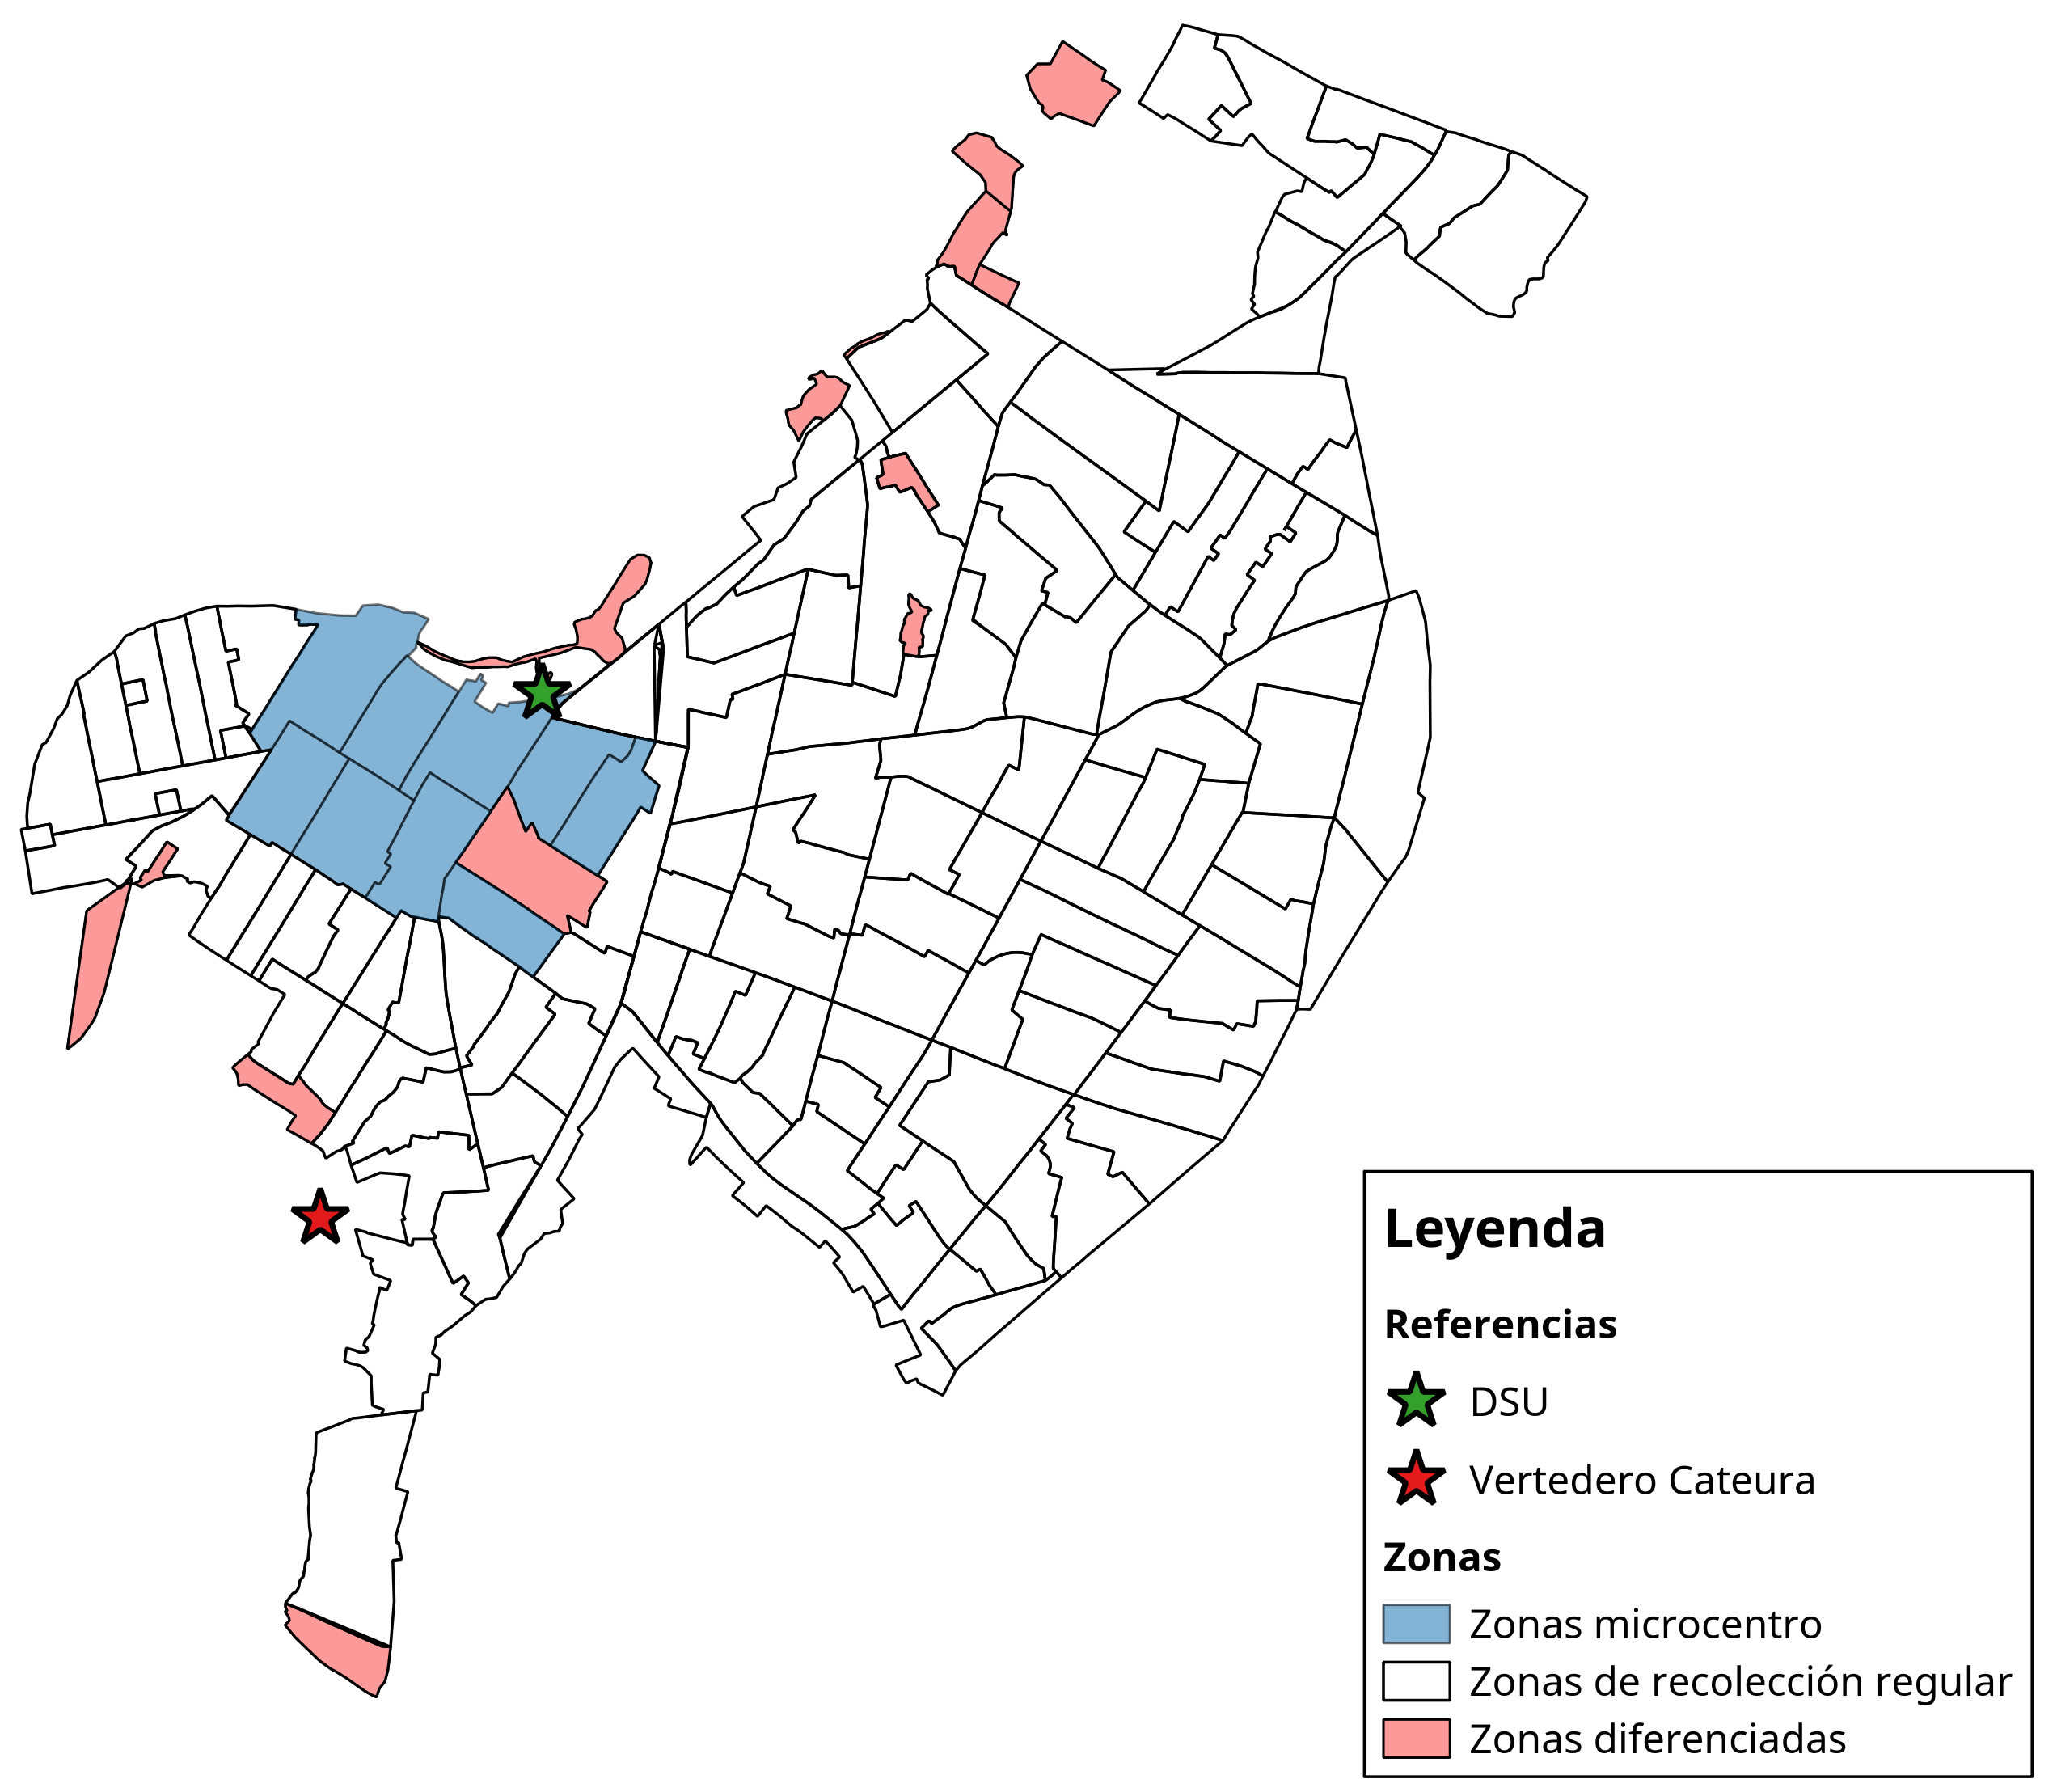
\includegraphics[width=8.5cm]{imagenes/Recoleccion-ZONAS_CUADRANTES.png}}
\caption{División de la ciudad en zonas. Un turno está correspondido por un conjunto de zonas coloreadas del mismo color. [Fuente: Departamento de Recolección de la DSU].}
\label{fig:zonasRecoleccion}
\end{figure}

\subsection{Colección de Datos}

En la ``Fig.~\ref{fig:metodologia}'' se muestra la metodología seguida en este trabajo: la recolección de datos, el modelado matemático, la implementación de la herramienta \textit{TapeYty}, el despliegue de la ruta óptima y por último el análisis de los resultados.

\begin{figure}[tbp]
\centerline{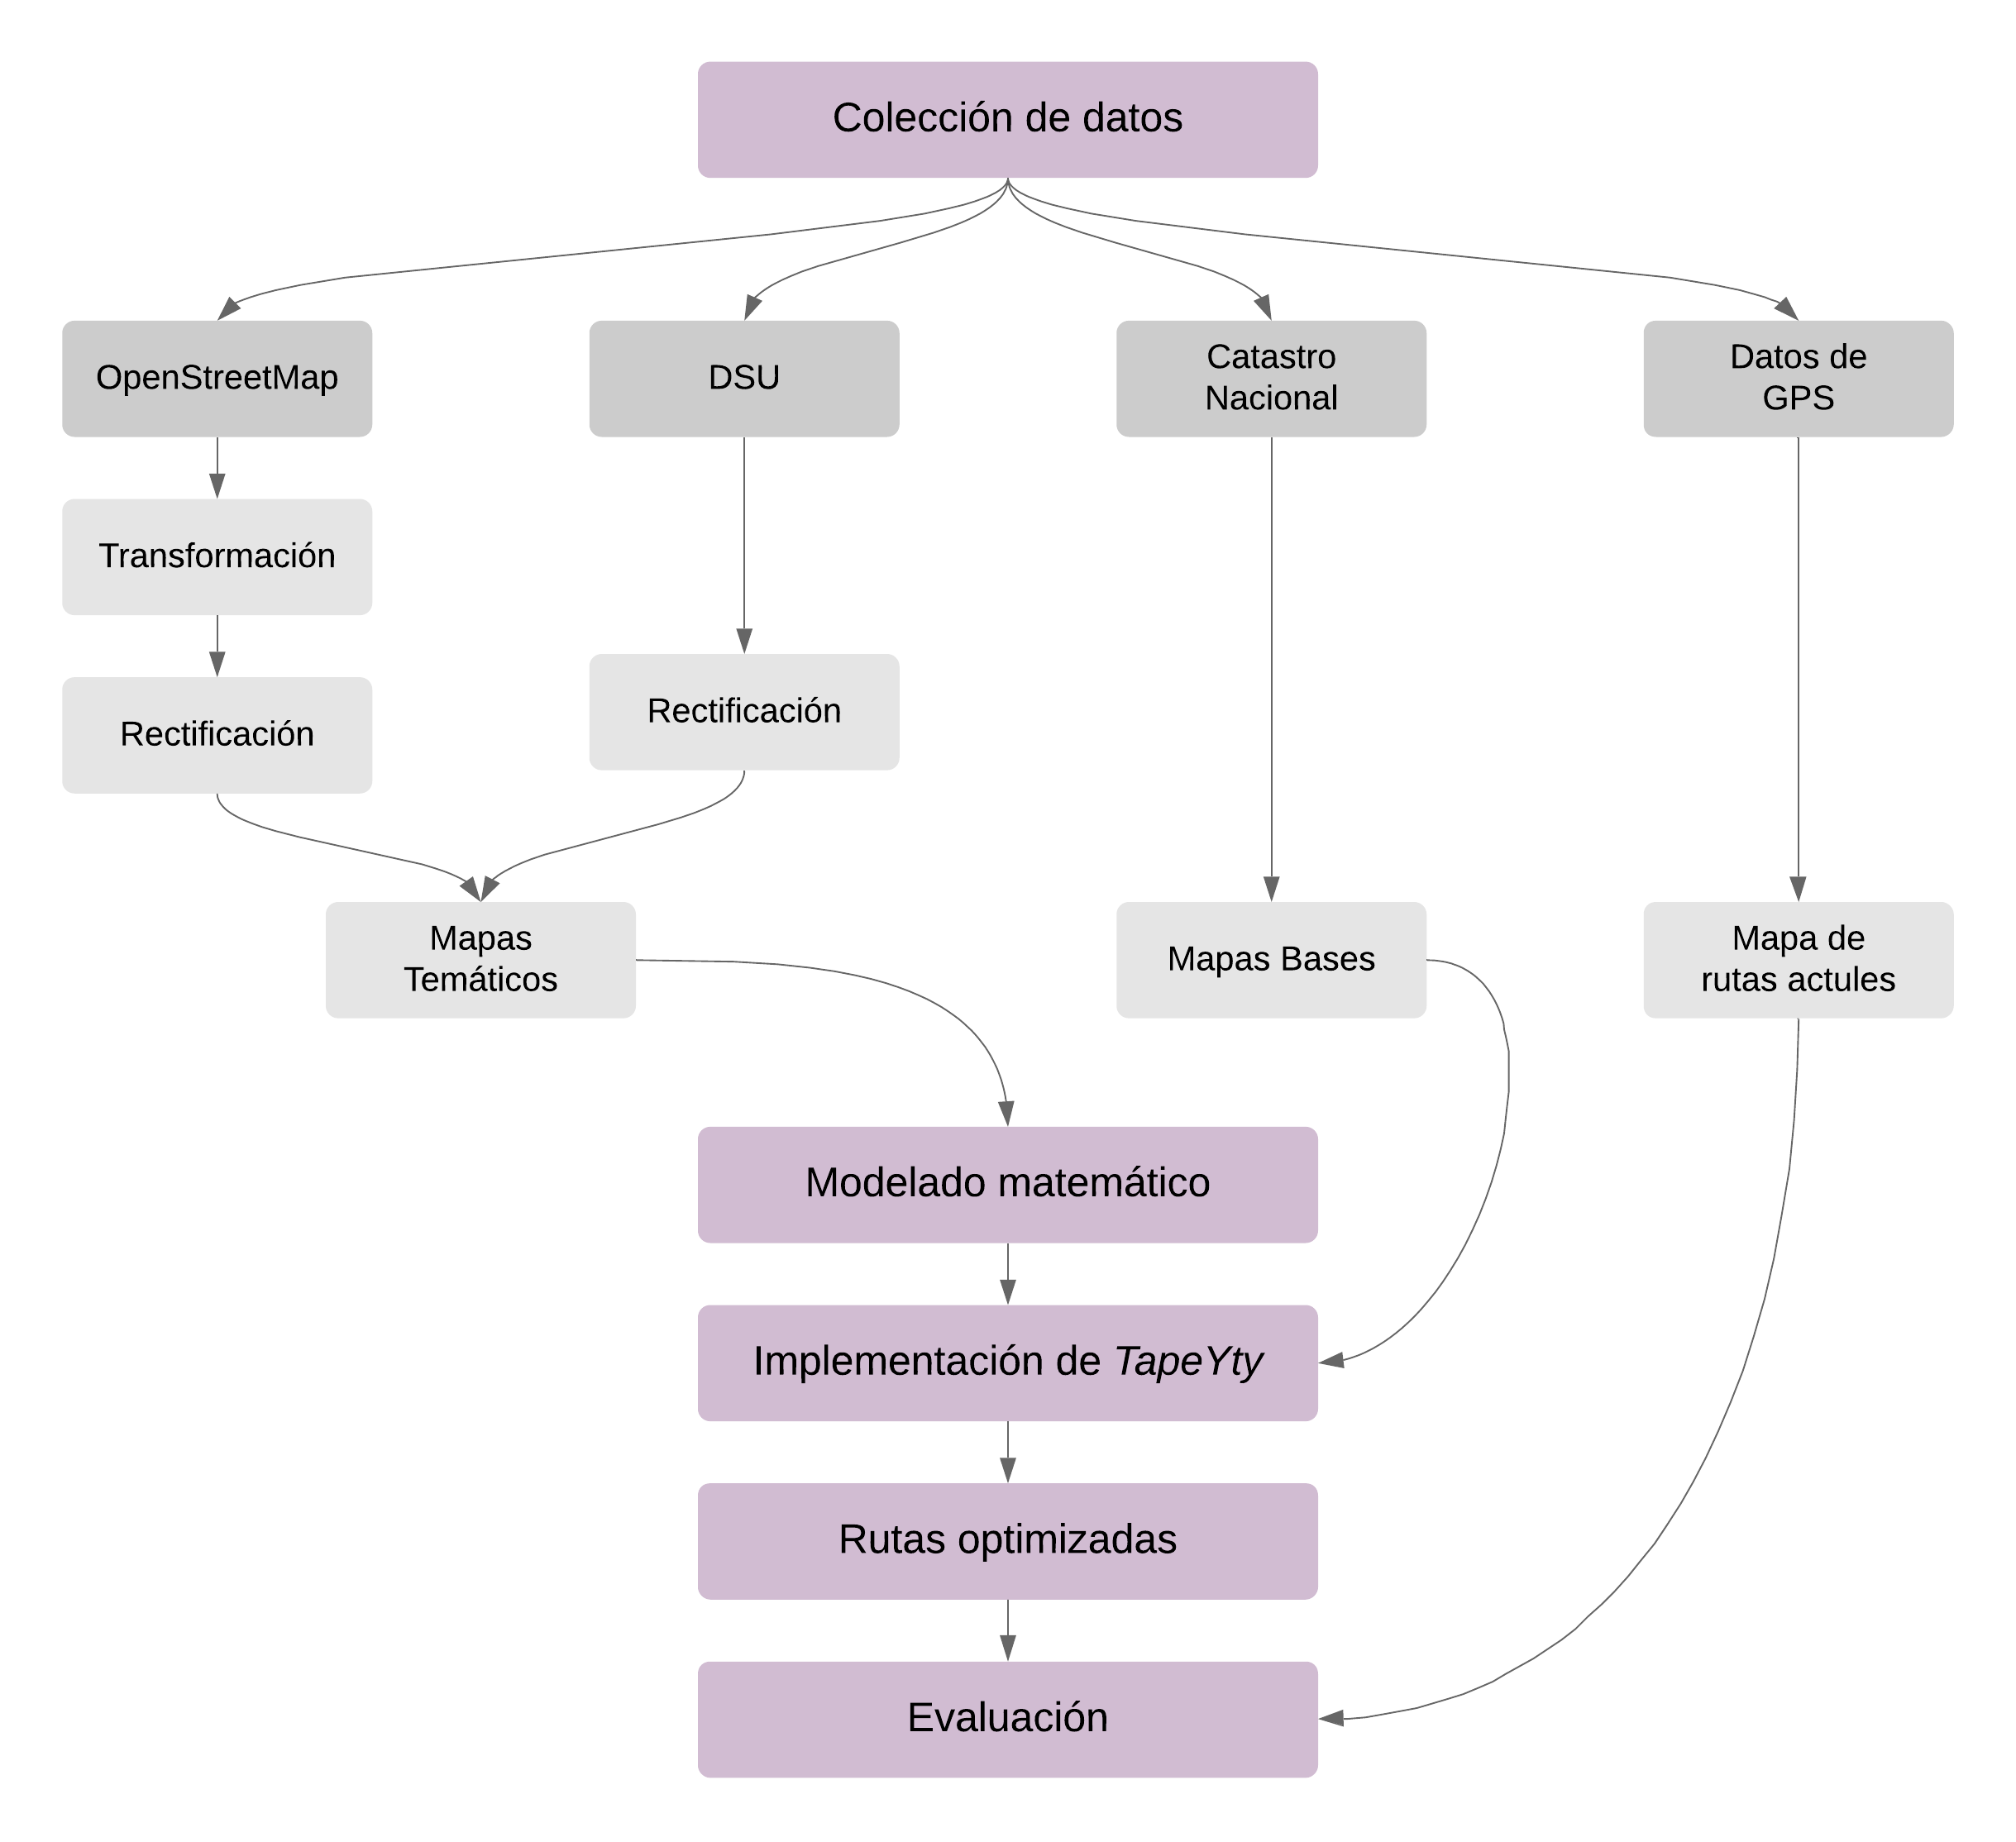
\includegraphics[width=9.5cm]{imagenes/DiagramaDeMetodologia.png}}
\caption{Procedimientos de la metodología.}
\label{fig:metodologia}
\end{figure}

Se crea una base de datos espacial utilizando el gestor de base de datos de código abierto PostgreSQL \cite{PostgreSQL}, junto con su extensión PostGIS \cite{PostGIS} que brinda soporte de objetos geográficos.

Se necesitó exportar los datos de Asunción desde \textit{OpenStreetMap} (OSM) \cite{OpenStreetMap}, debido a que no se tuvo conocimiento de alguna institución que proveyera de mapas de calles de la ciudad con sus sentidos. Se utiliza la herramienta \textit{osm2pgsql} para importar los datos de OSM a la base de datos, en el sistema de referencia geográfico WGS84 (SRID 4326). Se utilizan las funciones de PostGIS para convertir los valores de latitud y longitud al tipo de dato geométrico \textit{Point}, es decir, un Punto. Se excluyen los puntos que no pertenecen a calles de la ciudad, además de puntos superpuestos. Las calles de OSM están representadas por líneas, que a su vez contienen una serie de nodos (puntos). Para un mejor manejo de la red de rutas se crea un proceso de segmentación de las calles, donde cada segmento de calle está formado por pares de nodos consecutivos, se define el sentido del segmento, longitud y si el segmento de calle es un callejón sin salida. Posteriormente se realizan las transformaciones correspondientes para almacenar las restricciones de giro y contramano.

La delimitación de las zonas de recolección fue proveída por la DSU a través de un archivo \textit{shape} del tipo de dato geométrico Polígono, que se importa a la base de datos mediante la herramienta \textit{shp2pgsql}. Se usa el sistema QGIS \cite{QGISSite} para la limpieza y correción de datos geográficos. El Servicio Nacional de Catastro (SNC) \cite{SNC} provee los mapas bases de Departamentos y Distritos a la aplicación a través de su portal de datos abiertos. Además, la DSU cuenta en  algunos  vehículos  de  su  flota con un sistema de monitoreo mediante el Sistema de Posicionamiento Global (GPS, \textit{Global Positioning System}). Se accede a los datos a través de archivos en formato de plantillas para su posterior importación a la base de datos.

\subsection{Modelo matemático}

Como resultado de la revisión del estado del arte, se utiliza la solución propuesta por Braier et al. \cite{Braier2017AnArgentina} para optimizar el enrutamiento de vehículos recolectores, ya que este modelo contempla las restricciones de la red de rutas, resolviendo una de las debilidades de los enfoques de la programación matemática mencionado en \cite{Sulemana2018OptimalMethods}. Además, la falta de datos relacionados con la cantidad de toneladas recolectadas por zonas fue otro de los principales motivos por el cual se seleccionó un problema de ruta cuya demanda se encuentra sobre los arcos (calles que deben ser visitadas), y además no posea restricciones de capacidad.

El estudio en \cite{Braier2017AnArgentina} presenta similitudes con el caso de estudio de este trabajo, entre ellas es posible citar:

\begin{itemize}
    \item División de la ciudad en sectores y recolección casa por casa: La situación es muy similar, ya que el procedimiento consiste en recoger los residuos domiciliarios casa por casa, debiendo cubrir todas las calles de un conjunto de cuadras o manzanas, denominadas zonas.
    \item Tamaño de problema: Una zona de recolección abarca en promedio el mismo número (entre 40 y 80 cuadras aproximadamente).
    \item Calles, carreteras, caminos: el trabajo \cite{Braier2017AnArgentina} tomó como caso de estudio la ciudad de Morón el cual presenta caminos con particularidades muy comunes a otras sudamericanas como la de Asunción, calles sin salida, calles estrechas, peatonales, giros prohibidos, entre otros.
\end{itemize}

Cada zona de recolección de la ciudad de Asunción es representada por un grafo mixto $H$ \cite{Braier2017AnArgentina}, cuyos nodos representan las esquinas de las calles en la zona, y los arcos son los segmentos de calles que corren entre dos intersecciones consecutivas. Las calles de un único sentido están representadas por arcos dirigidos y las calles finas de doble sentido por arcos no dirigidos, ya que ambos lados de la calle pueden ser servidos en un solo viaje. En el caso de calles anchas de doble sentido, como las avenidas, cada lado debe ser servido de forma separada, por lo que estas calles se representan con dos arcos dirigidos, una en cada sentido.

Para incorporar las restricciones de regulación de tráfico se construye un grafo dirigido $G$ desde el grafo $H$. El grafo $H$ es expandido dividiendo cada nodo en varios nuevos nodos representando todas las formas en las que se puede llegar y salir de la esquina en cuestión. En la ``Fig.~\ref{fig:grafo_expandido}(a)'' se puede observar un nodo en el grafo original $H$ antes de su expansión, y en la ``Fig.~\ref{fig:grafo_expandido}(b)'' el nodo que ha sido expandido en seis nuevos nodos, representando cada posible entrada y salida del nodo. Los arcos auxiliares dirigidos son agregados y conectan los nuevos nodos, representando así las transiciones permitidas de una esquina a otra.

El modelo de programación entera propuesto por \cite{Braier2017AnArgentina} está definido de la siguiente manera:

\subsubsection{Conjuntos y Parámetros}
\label{sec:conjunto-parametros}

\begin{itemize}
\item $G(V, A)$: Grafo dirigido en el que los nodos V corresponden a todas las alternativas posibles para llegar a las esquinas de las intersecciones y A está compuesto por arcos que se pueden atravesar en una sola dirección específica.

\item $E \subseteq \{ \{i, j\}: i \in V, j \in V, i \neq j\}$: Representan segmentos de calles de dos vías que pueden ser recorridos en cualquier sentido.

\item $AM \subseteq A $: Arcos obligatorios que representan segmentos que deben recorrerse únicamente en el sentido especificado.

\item $w : A \rightarrow \mathbb{R} $: Función de peso que asocia un peso a cada arco, en este caso la distancia del segmento de calle. Los arcos auxiliares entre nodos que representan esquinas tienen un mismo valor ínfimo.

\item $I \subseteq V $: Nodos que especifican los puntos de inicio permitidos para la ruta.

\item $S \subseteq V$: Se define $\delta^+ (S) = \{i j \in A: i \in S , j \notin S \}$ , que representa un conjunto de arcos que van desde nodos en $S$ a nodos en $V \backslash S$.
\end{itemize}

El problema de ruteo es una versión particular del problema del cartero rural abierto dirigido generalizado, ya que el arco $i j \in E $ determina el grupo de arcos $L_{i j} = \{i j, j i\}$, en el que al menos uno de ellos debe ser atravesado en la solución final y además se busca un camino cuyo nodo inicial y final no se especifican.

\begin{figure}[tbp]
\centerline{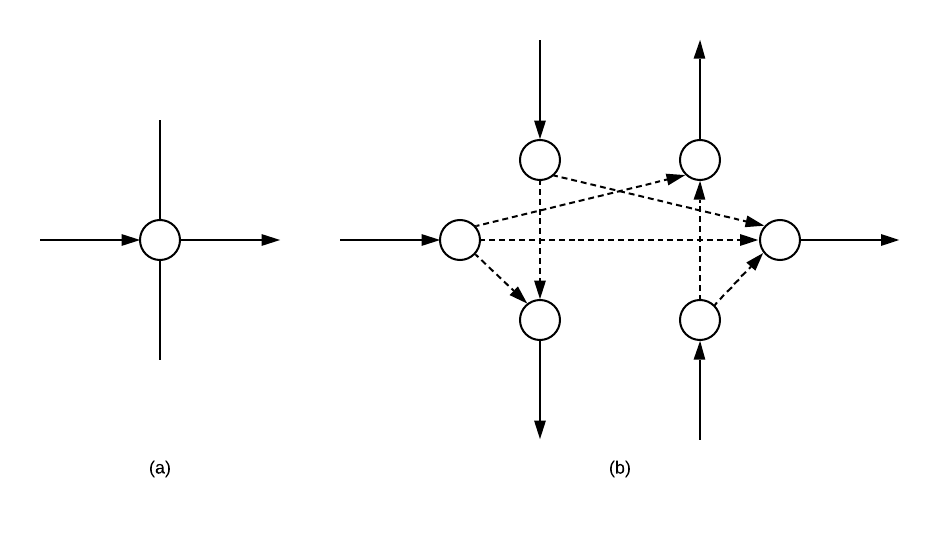
\includegraphics[width=9.5cm]{imagenes/expanded_graph.png}}
\caption{Expansión de un cruce entre una calle de sentido único y una calle de doble sentido. (a) Grafo mixto original. (b) Grafo dirigido luego de la expansión, los arcos auxiliares están representados por líneas discontinuas. \cite{Braier2017AnArgentina}}
\label{fig:grafo_expandido}
\end{figure}

\subsubsection{Variables de decisión}
\begin{itemize}
\item $x_{i j}$: Para cada arco $ {i j} \in A$ esta variable representa el número de veces que $i j$ es atravesado.

\item $s_i$: Para cada nodo $i \in I$ esta variable binaria especifica si  $i$ es el primer nodo de la ruta.

\item $t_j$: Para cada nodo $j \in V$ esta variable binaria indica si $j$ es el último nodo de la ruta.
\end{itemize}

\subsubsection{Definición del programa entero}
\label{sec:programa-entero}
\begin{equation} \tag{0} \label{eq0}
\min \sum_{i j \in A} w_{i j} x_{i j}  \\
\end{equation} 
\hbox{}

\begin{equation} \tag{1} \label{eq1}
\begin{gathered}
x_{i j} \geq 1 \\
\forall i j \in A M
\end{gathered}
\end{equation} 
\hbox{}

\begin{equation} \tag{2} \label{eq2}
\begin{gathered}
x_{i j} + x_{j i} \geq 1 \\
\forall i j \in E
\end{gathered}
\end{equation}
\hbox{}

%ecuacion 3a
\begin{equation} \tag{3a} \label{eq3a}
\begin{gathered}
s_i + \sum_{j: j i \in A} x_{j i} = \sum_{j: i j \in A} x_{i j} + t_i \\
\forall i \in I
\end{gathered}
\end{equation} 
\hbox{}

%ecuacion 3b
\begin{equation} \tag{3b} \label{eq3b}
\begin{gathered}
\sum_{j: j i \in A} x_{j i} = \sum_{j: i j \in A} x_{i j} + t_i \\
\forall i \in V\backslash I
\end{gathered}
\end{equation}
\hbox{}

\begin{equation} \tag{4} \label{eq4}
\sum_{i \in I} s_i = 1 
\end{equation}
\hbox{}

\begin{equation} \tag{5} \label{eq5}
\sum_{i \in V} t_i = 1 
\end{equation}
\hbox{}

\begin{equation} \tag{6} \label{eq6}
\begin{gathered}
    \sum_{i j \in \delta + (S)} x_{i j} \geq 1 \\
    \forall S \subseteq V
\end{gathered}
\end{equation}
\hbox{}

\begin{equation} \tag{7} \label{eq7}
\begin{gathered}
    x_{i j} \in \mathbb{Z}_+ \\
    \forall i j \in A
\end{gathered}
\end{equation}
\hbox{}

\begin{equation} \tag{8} \label{eq8}
\begin{gathered}
    s_i \in \{0,1\} \\
    \forall i \in I
\end{gathered}
\end{equation}
\hbox{}

\begin{equation} \tag{9} \label{eq9}
\begin{gathered}
    t_i \in \{0,1\} \\
    \forall i \in V
\end{gathered}
\end{equation}

La función objetivo (\ref{eq0}) busca minimizar el costo total de la ruta de recolección de residuos. El costo en este trabajo se refiere a la distancia recorrida por el vehículo recolector. La restricción (\ref{eq1}) impone que todos los arcos de único sentido deben ser visitados al menos una vez, la (\ref{eq2}) requiere que los arcos no dirigidos sean atravesados al menos una vez en cualquier sentido. Las restricciones (\ref{eq3a}) y (\ref{eq3b}) aseguran que la solución encontrada es realmente un camino agregando la condición de conservación de flujo estándar a cada nodo. Las restricciones (\ref{eq4}) y (\ref{eq5}) garantizan que el nodo inicial y final sean únicos. Las restricciones (\ref{eq1})-(\ref{eq5}) permiten la formación de subtours, la restricción (\ref{eq6}) es el estándar de eliminación de subtours. Las restricciones (\ref{eq7})-(\ref{eq9}) especifican los valores posibles para las variables del modelo.

\subsubsection{Algoritmo de solución}
\label{algoritmo-solucion}
En el modelo dado en la sección \ref{sec:programa-entero} se puede observar la restricción de eliminación de subtours la cual es muy costosa en la generación de las mismas como también en  la complejidad del problema. En este contexto la estrategia propuesta en \cite{Braier2017AnArgentina} se basa en tratar de obtener una solución rápidamente sin considerar el problema de subtour e ir agregando las restricciones sucesivamente, esto se conoce como técnica de agregación dinámica de restricciones a un modelo relajado.

Los siguientes pasos detallan la estrategia:

\begin{enumerate}
\item Crear el modelo relajado $M: = (\ref{eq1}) - (\ref{eq5})$ y $(\ref{eq7}) - (\ref{eq9})$.
\item Resolver $M$.
\item Si no se puede encontrar ninguna solución para $M$, retornar ``infactible'' y parar.
\item Si la mejor solución encontrada para $M$ no tiene subtours, retornar esta solución y parar.
\item Si los subtours pueden ser mezclados con el tour que contiene el nodo inicial y final, entonces mezclarlos, retornar la solución obtenida y parar.
\item De lo contrario, agregar a $M$ la restricción de eliminación de subtour estándar (\ref{eq6}) por cada subtour en la solución y regresar al paso 2.
\end{enumerate}

\subsection{Método de secuenciación}

En este trabajo se utiliza el algoritmo implementado en \cite{RiveraHazim2015APath} que encuentra el camino euleriano de un multigrafo dirigido para obtener la secuencia a seguir. Se genera un multigrafo dirigido $MG$ a partir del resultado del problema descrito en la sección anterior, creando arcos dirigidos según la cantidad de veces que se atraviesa por cada arco del grafo $G$. 

El algoritmo recibe como parámetros de entrada el nodo inicial, nodo final y $MG$. Devuelve como resultado, la secuencia de arcos del recorrido solución. La complejidad del algoritmo es $O(N + M)$, donde $N$ es el número de vértices y $M$ es el número de arcos.

\subsection{Ejemplo Numérico}
A continuación se describe un ejemplo simple de como la aplicación produce la secuencia del camino a seguir desde el resultado generado por la programación matemática.

El Paso 1 de la ``Fig.~\ref{fig:PasosSolucion}'' muestra los datos de salida que genera el modelo matemático (Algoritmo  de  solución, sección \ref{algoritmo-solucion}) a partir de un resultado factible. La salida contiene todos los segmentos que son utilizados como solución junto con el número de veces que se recorre cada uno de ellos, así como también despliega los nodos que resultaron elegidos como nodo inicial y nodo final del recorrido. Posteriormente, con estos datos se procede a crear el multigrafo dirigido $MG$ con la cantidad total de arcos resultantes (Paso 2). El multigrafo generado pasa a formar parte de la entrada para obtener la secuencia del camino a seguir (Paso 3). Por último, el algoritmo de secuenciación se resuelve y genera como salida la secuencia de arcos del algoritmo de optimización.

\begin{figure*}[htbp]
\centerline{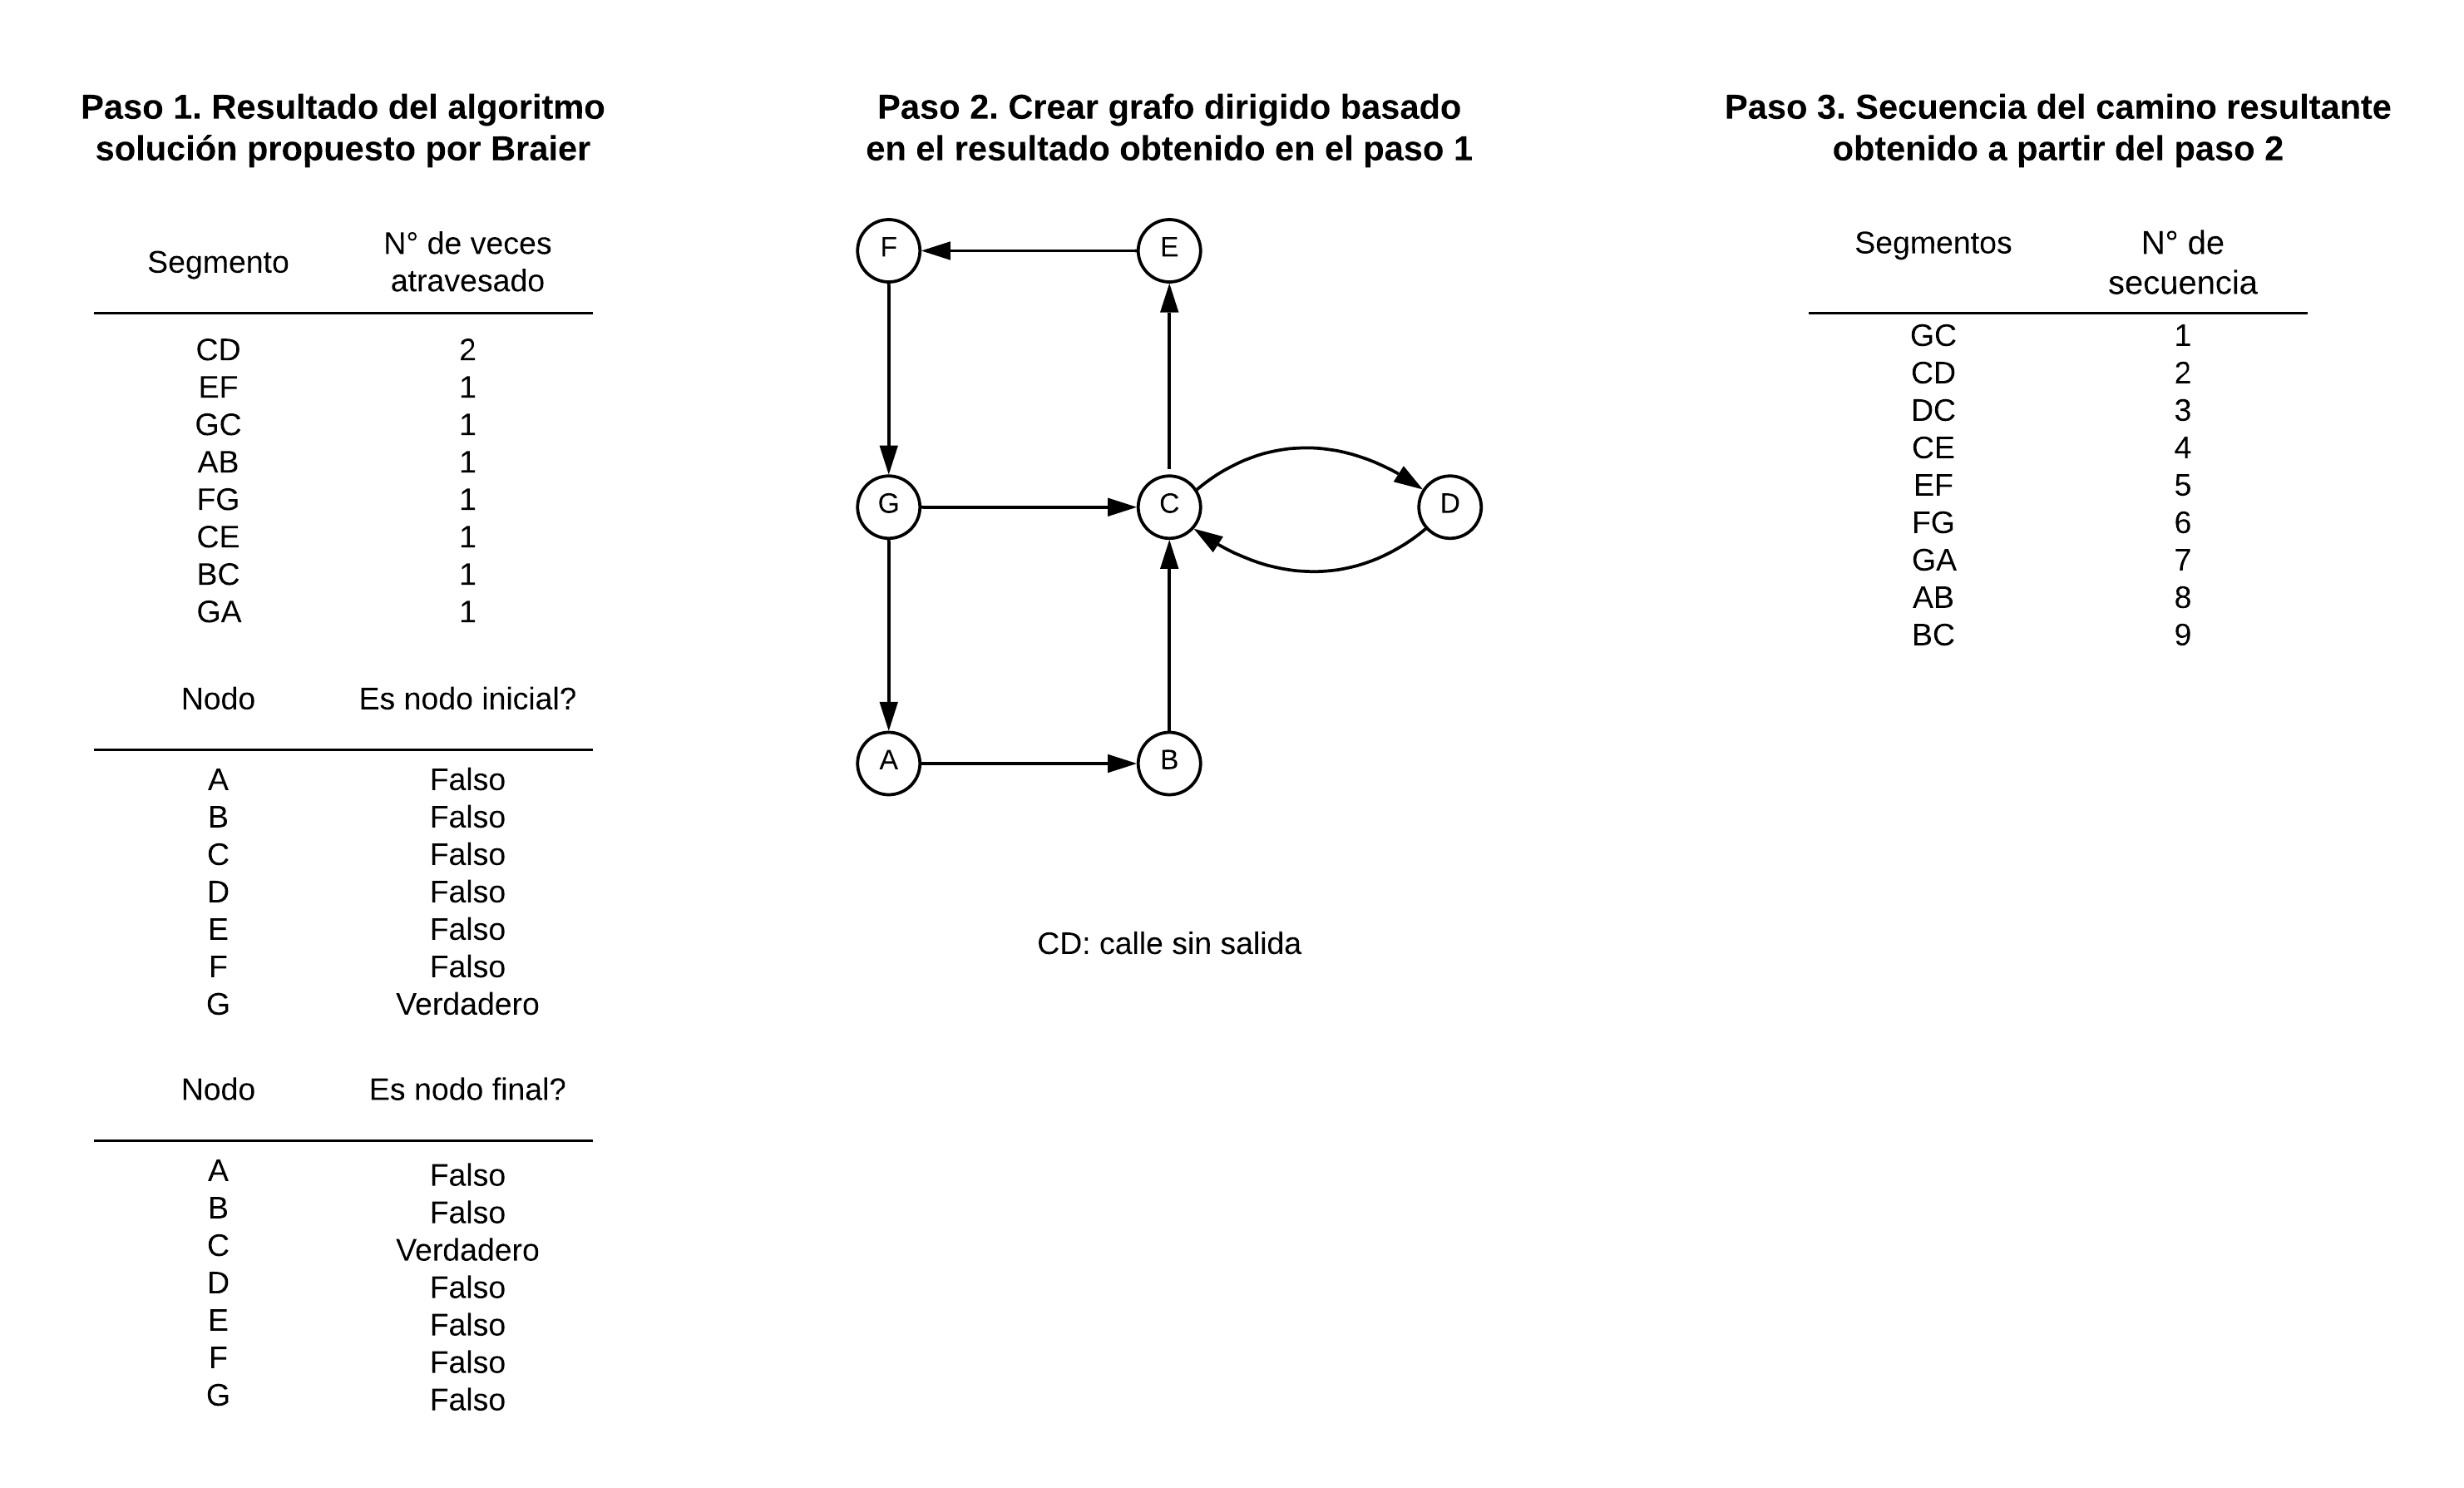
\includegraphics[width=0.82\textwidth]{imagenes/pasos_de_solucion.png}}
\caption{Pasos de solución para obtener la secuencia del camino del vehículo recolector en una zona.}
\label{fig:PasosSolucion}
\end{figure*}

\subsection{Solución propuesta}

En la actualidad, la DSU no cuenta con un \textit{software} que apoye a la toma de decisiones en lo que respecta a la gestión de residuos sólidos urbanos, más específicamente en el área de recolección. Se propone la implementación de una herramienta GIS que contribuya con la elección de mejores caminos a seguir por los vehículos recolectores, y de esta manera generar mayores beneficios en cuanto a tiempo y distancia, además de garantizar que el servicio sea brindado a todos los domicilios.
%además de contribuir con el cuidado del medio ambiente.

La ``Fig.~\ref{fig:disenhoArquitectura}'' muestra el diseño de la arquitectura de \textit{software} alrededor de la aplicación solución \textit{TapeYty}. Este diseño se divide en dos partes que se explicarán en detalle a continuación.

\subsubsection{Cliente}

Desde una computadora portátil o un teléfono móvil el usuario puede acceder a la aplicación e ingresar con sus credenciales desde el navegador (\textit{browser}). Se ejecuta en el navegador el código Javascript generado a partir del código fuente construido con el marco (\textit{framework}) Angular (versión 7.0) \cite{Angular}. Angular es un \textit{framework} ampliamente utilizado para el desarrollo de aplicaciones web con excelentes prestaciones en cuanto a rendimiento, escalabilidad, velocidad de respuesta y cuenta con una comunidad numerosa y activa. Una de las librerías incorporadas al proyecto cliente más relevante para el trabajo es Mapbox GL JS \cite{MapboxJS}, la cual ofrece funcionalidades relacionadas a mapas en el lado cliente, teniendo como gran atractivo su buen desempeño durante el tiempo de renderizado de los mapas y datos geográficos.

La implementación se puede resumir en los siguientes módulos:
\begin{itemize}
    \item Seguridad: El sistema comprende un mecanismo de autenticación basada en tokens JWT (\textit{JSON Web Tokens}). Se restringe acceso a la aplicación y a los servicios REST del servidor no autenticados.
    \item Administración: Comprende la gestión (listar, agregar, editar, eliminar) de usuarios, vehículos, turnos.
    \item GIS: Este módulo despliega el mapa con las diferentes capas (zona, calle, departamento, distrito) y permite el manejo de capas, la gestión de calles pudiendo actualizar el sentido de las mismas, inhabilitarlas (``Fig.~\ref{fig:tapeYtyCalles}''), agregar restricciones de giro o de continuar el sentido (contramano) (``Fig.~\ref{fig:tapeYtyRestricciones}''), generación de rutas, despliegue de resultado de ruta optimizada (``Fig.~\ref{fig:RecorridoTapeYtyZona83Opcionales}''), entre otros.
\end{itemize}

\begin{figure*}[htbp]
  \centering
  \begin{subfigure}[b]{0.49\textwidth}
        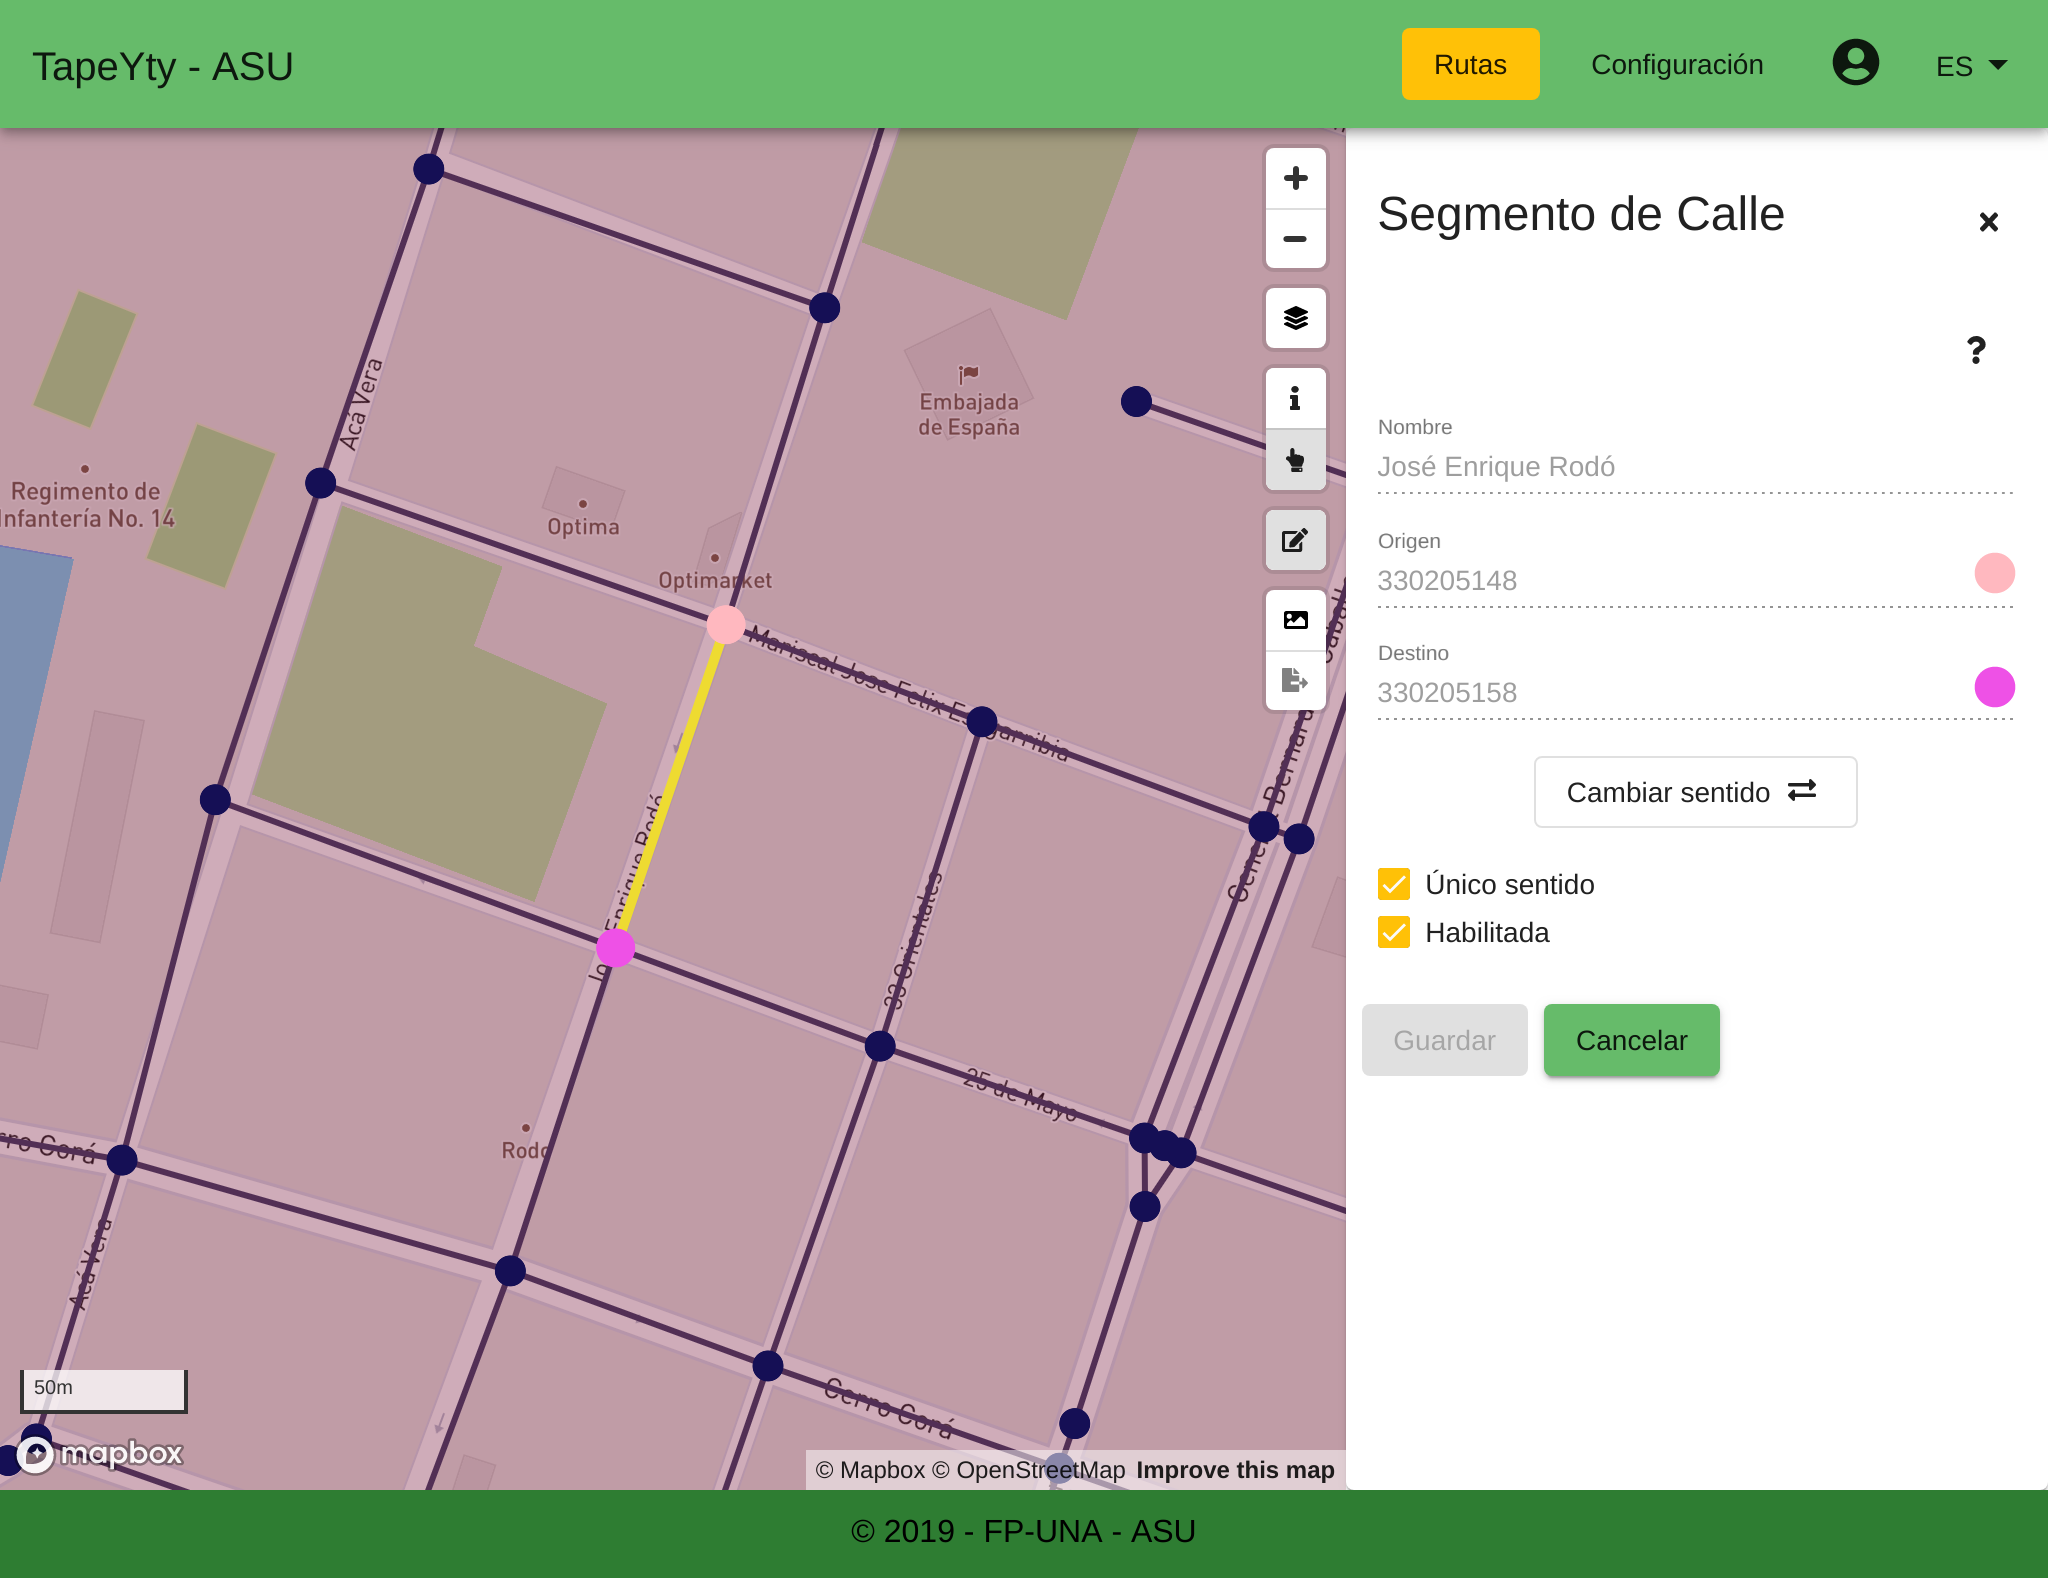
\includegraphics[width=\textwidth]{imagenes/segmento_calle.png}
        \caption{Gestión de calles}
        \label{fig:tapeYtyCalles}
  \end{subfigure}
   \begin{subfigure}[b]{0.49\textwidth}
        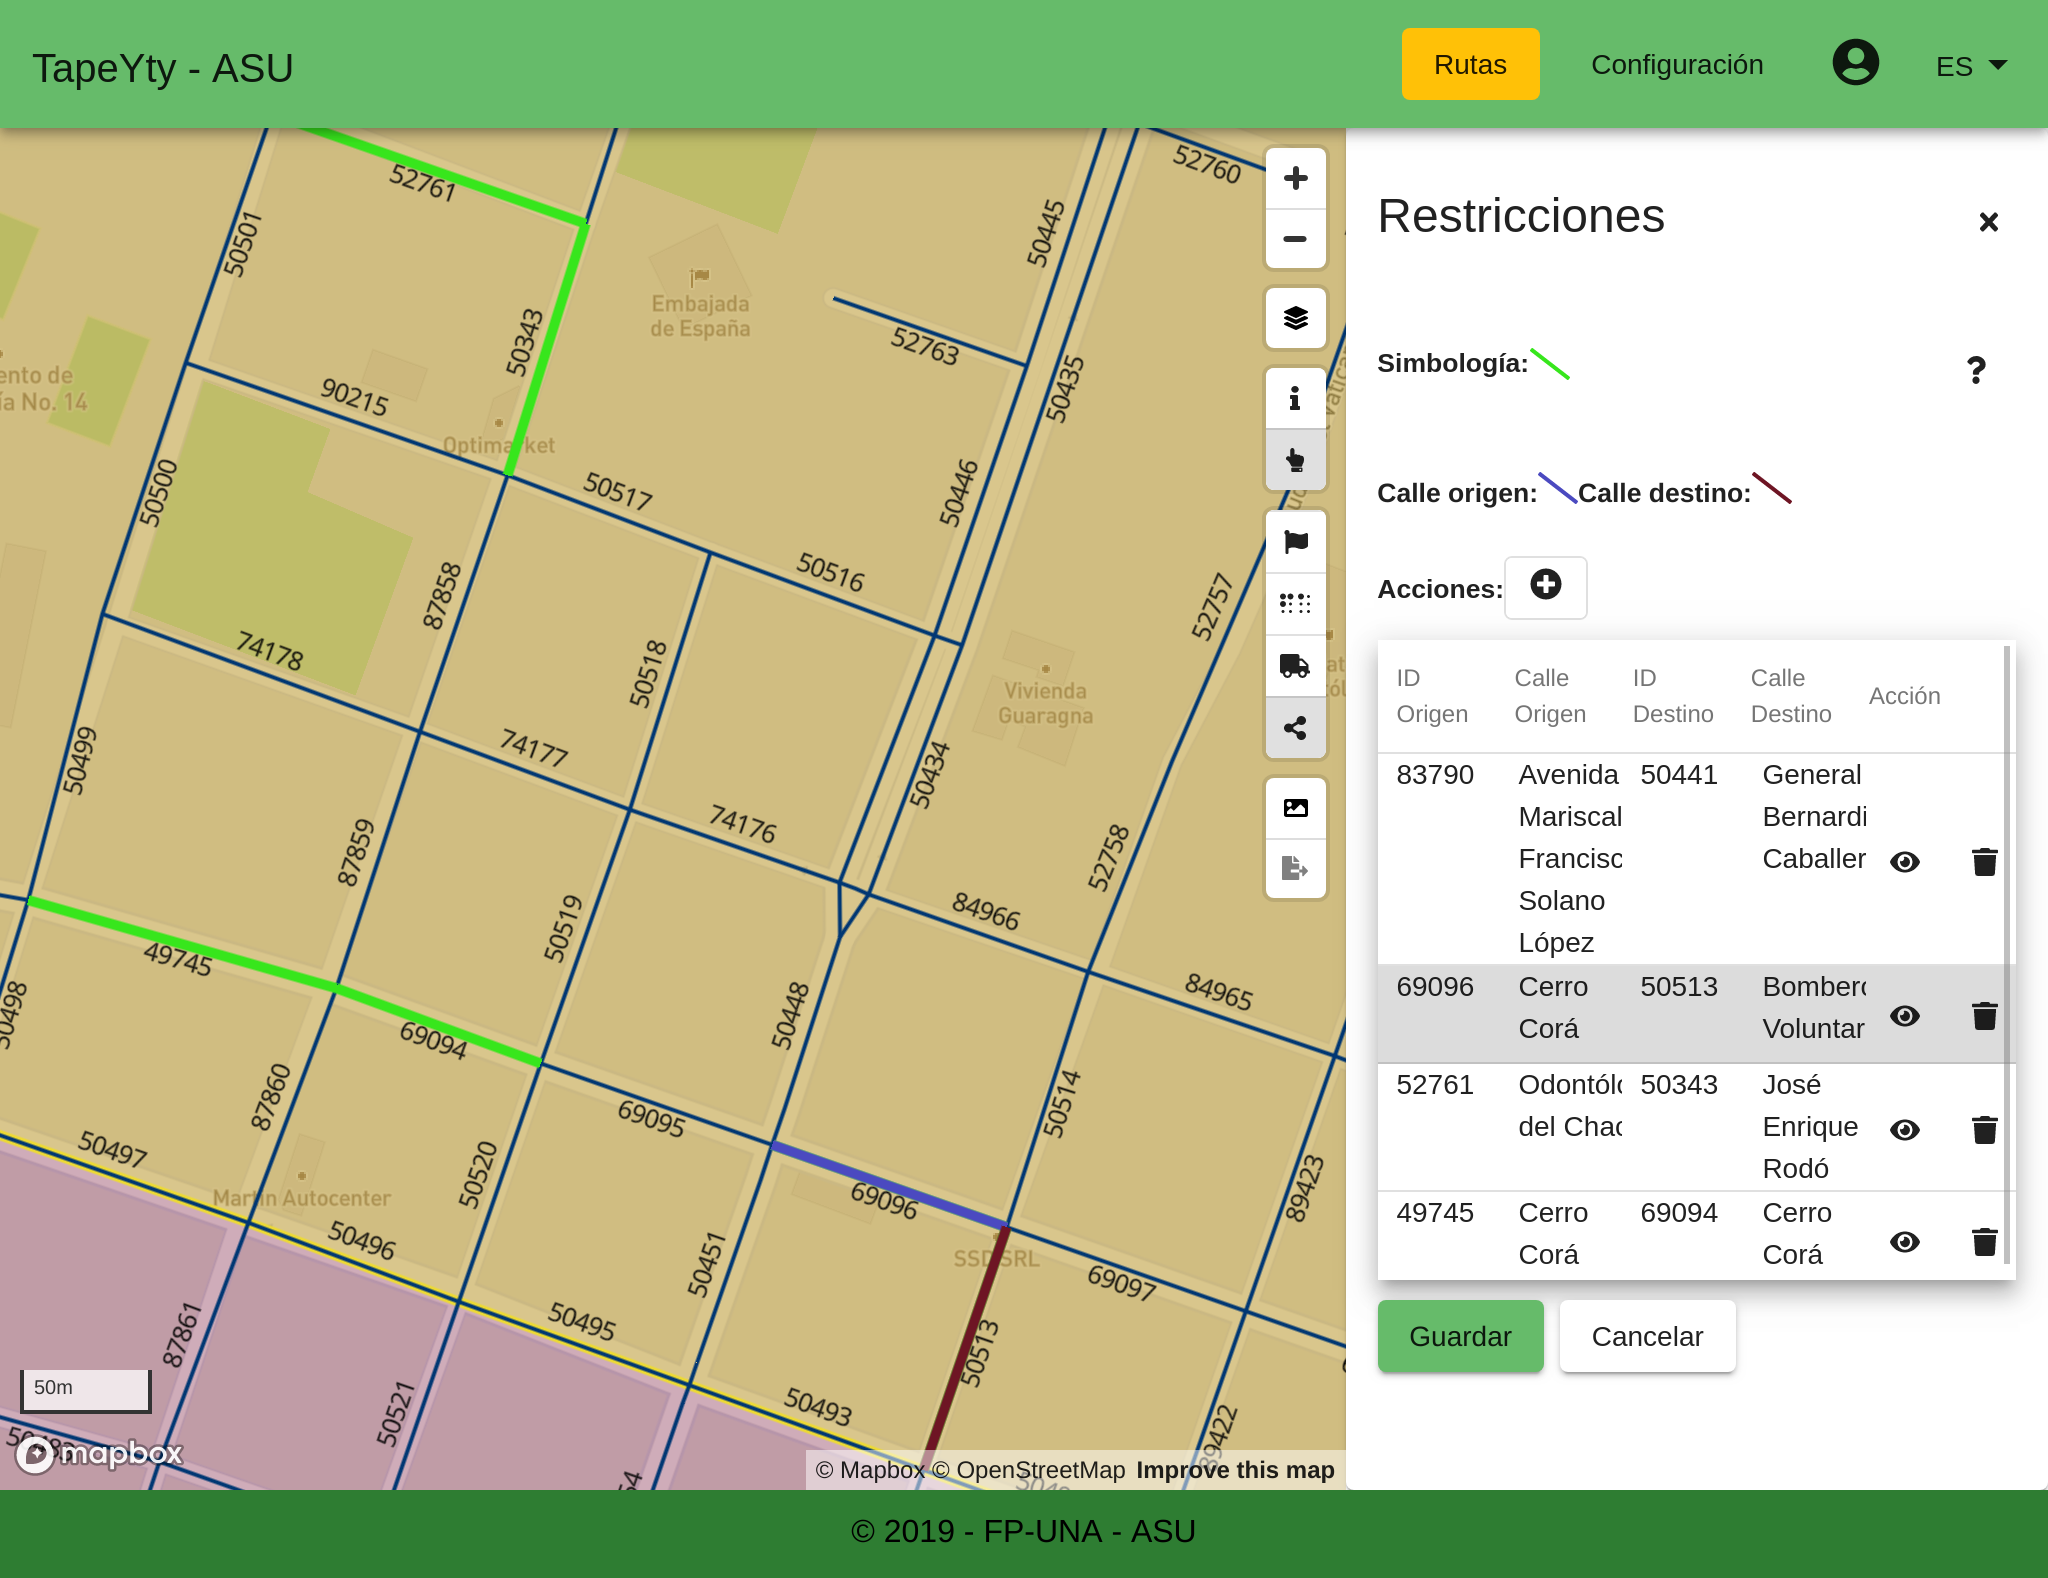
\includegraphics[width=\textwidth]{imagenes/restricciones.png}
        \caption{Gestión de restricciones}
        \label{fig:tapeYtyRestricciones}
  \end{subfigure}
  \caption{Aplicación \textit{TapeYty}}
\end{figure*}

\begin{figure}[tbp]
\centerline{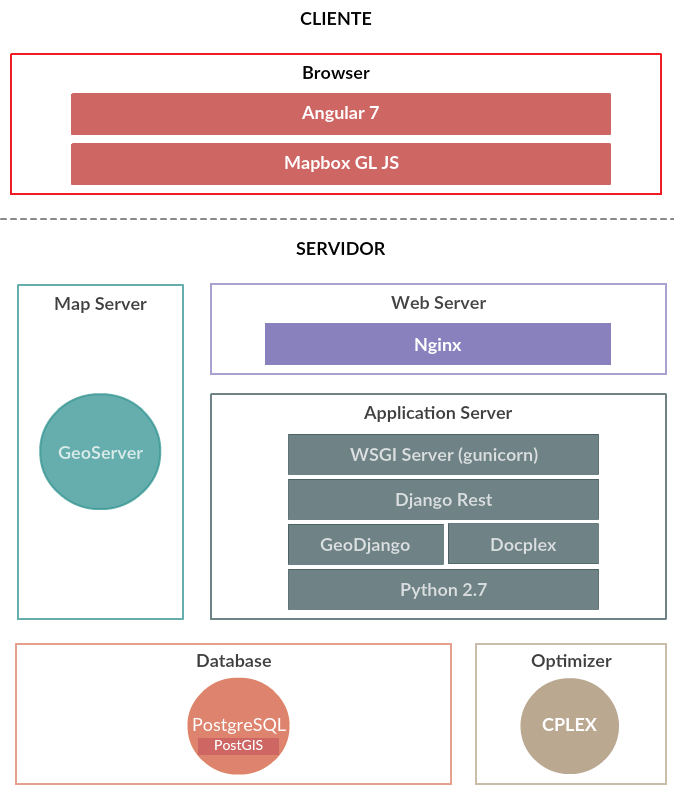
\includegraphics[width=7.6cm]{imagenes/20190424_WebAppArchitectureDesign.png}}
\caption{Diseño de arquitectura de \textit{TapeYty}.}
\label{fig:disenhoArquitectura}
\end{figure}

\subsubsection{Servidor}

El lado servidor presenta mayor complejidad ya que concentra varios componentes que además deben interactuar unos con otros.

Como parte de la solución, se utiliza PostgreSQL (v10.8) con su extensión PostGIS (v2.4), donde están almacenadas las distintas informaciones obtenidas, geográficas o no, excepto los datos (\textit{shapes}) que provienen del SNC de Paraguay.

El servidor de mapas GeoServer \cite{GeoServer} consiste en un servidor de código abierto que permite a los usuarios compartir y editar datos espaciales. En él se almacenan los mapas de Departamentos y Distritos del Catastro Nacional. Además, se crea una conexión con la base de datos para poner a disposición los mapas de calles y zonas, en modo lectura, donde el servidor ofrece servicios web de mapas como por ejemplo \textit{TMS} (\textit{Tile Map Service}), servicio que maneja estrategias de caché de cuadros de imágenes para mostrar los mapas con mayor velocidad dando un mejor rendimiento a la aplicación.

Para resolver el modelo seleccionado se requiere de un \textit{software} especializado para ello. Se opta por la herramienta \textit{CPLEX Optimizer} de IBM \cite{CPLEXOptimizer} en su versión académica, ya utilizada en trabajos previos como \cite{Vecchi2016ACollection,Ramos2018TheApproaches,BabaeeTirkolaee2019DevelopingStudy}. El modelo matemático puede ser codificado en CPLEX con el lenguaje OPL ({\textit{Optimization Programming Language}}), provee además interfaces C, C++, Java y Python para su modelado. Sin embargo, estas interfaces no son usadas directamente para modelar sino a través de la librería Docplex \cite{Docplex}.

Para el desarrollo propio de una aplicación web una de las preocupaciones más importantes es la elección del lenguaje y el \textit{framework} sobre los cuales estará construida. En este trabajo se opta por el lenguaje Python, conjuntamente con el framework GIS GeoDjango \cite{GeoDjango}. En el área GIS, Python es uno de los lenguajes más utilizados a lo largo del tiempo, pudiéndose encontrar muchas funciones, librerías, \textit{software}, entre otros; escritos con este lenguaje. GeoDjango, basado en Django, tiene la virtud de ser robusto, provee un modelo de programación MVC (\textit{Model-View-Controller}) y facilita el desarrollo de aplicaciones Web. 

La librería Docplex de Python resulta en una sencilla integración con nuestro \textit{framework}, también permite formular el modelo de forma clara y directa en comparación con las interfaces de CPLEX, resultando muy similar a la formulación con el lenguaje OPL.

Con Docplex y GeoDjango se implementa toda la lógica de negocio de la aplicación. Para poder acceder a esta lógica desde el cliente se requiere de una API (\textit{Application Programming Interface}). Para ello, se utiliza el protocolo de comunicación de intercambio de datos RESTful con la librería Django REST Framework y Django Rest Framework GIS. Se implementan los servicios para los módulos citados anteriormente como: agregar, eliminar y editar usuarios, editar propiedades alfanuméricas de calles, generar la ruta óptima de una zona, entre muchos otros; con estructuras de datos en formato JSON y geoJSON.

Finalmente, se prepara el ambiente de producción para su implantación. Se instala el servidor web Nginx \cite{NGINX} que recibe una solicitud HTTP del cliente (el navegador), interpreta la solicitud y la envía a la puerta de enlace (\textit{gateway}) Gunicorn \cite{Gunicorn}. Gunicorn es un servidor HTTP de Interfaz de Pasarela del Servidor Web de Python (WSGI, \textit{Web Server Gateway Interface}) que traduce la solicitud recibida del servidor web para que la aplicación pueda manejarla. Por último tenemos la aplicación que a través de su API recibe la petición para luego procesarla y responderla.

\section{Resultados y Discusiones}

En esta sección se presenta un análisis de los resultados obtenidos con \textit{TapeYty}. Se tomaron los datos del camino trazado por el GPS instalado en el vehículo recolector 129 en la zona 83 de trabajo con una distancia total recorrida de 16.940 km, donde se pudo observar que varios segmentos de calles fueron recorridos repetidas veces mientras que otros dentro de la zona no fueron atravesados. En la práctica, los recolectores suelen acumular las bolsas de basura de varias casas en una esquina, evitando que el conductor entrase a ciertas calles. Lastimosamente no se puede asegurar que dichos segmentos hayan recibido el servicio.

Las calles sin salida, las estrechas y las que limitan una zona pero que no deben ser visitadas necesariamente son gestionadas mediante \textit{TapeYty}. En el módulo de rutas de la aplicación el usuario tiene la posibilidad de modificar propiedades de las calles como ser el sentido, si se encuentra inhabilitada, o si es opcional el paso del camión por un segmento de calle determinado. Por ejemplo, en la ``Fig.~\ref{fig:RecorridoTapeYtyZona83Opcionales}'' ciertos segmentos de calles pasan a ser opcionales para el paso de camiones simulando el procedimiento llevado a cabo por el equipo de recolección de la zona 83. El punto de inicio de la ruta generada se representa en el mapa con un punto verde, el punto final con un punto rojo y la secuencia a seguir se encuentra especificada en los segmentos de calle. Algunos números de secuencia no son visibles en el mapa debido a que los segmentos son muy pequeños y se requiere de acercamiento para verlos, por ejemplo, el sexto segmento a atravesar no es visible debido a su longitud. El sistema permite exportar un archivo con formato GPX (\textit{GPS eXchange Format}) de la ruta generada que es utilizada para la navegación de la ruta.

\begin{figure*}[tbp]
\centerline{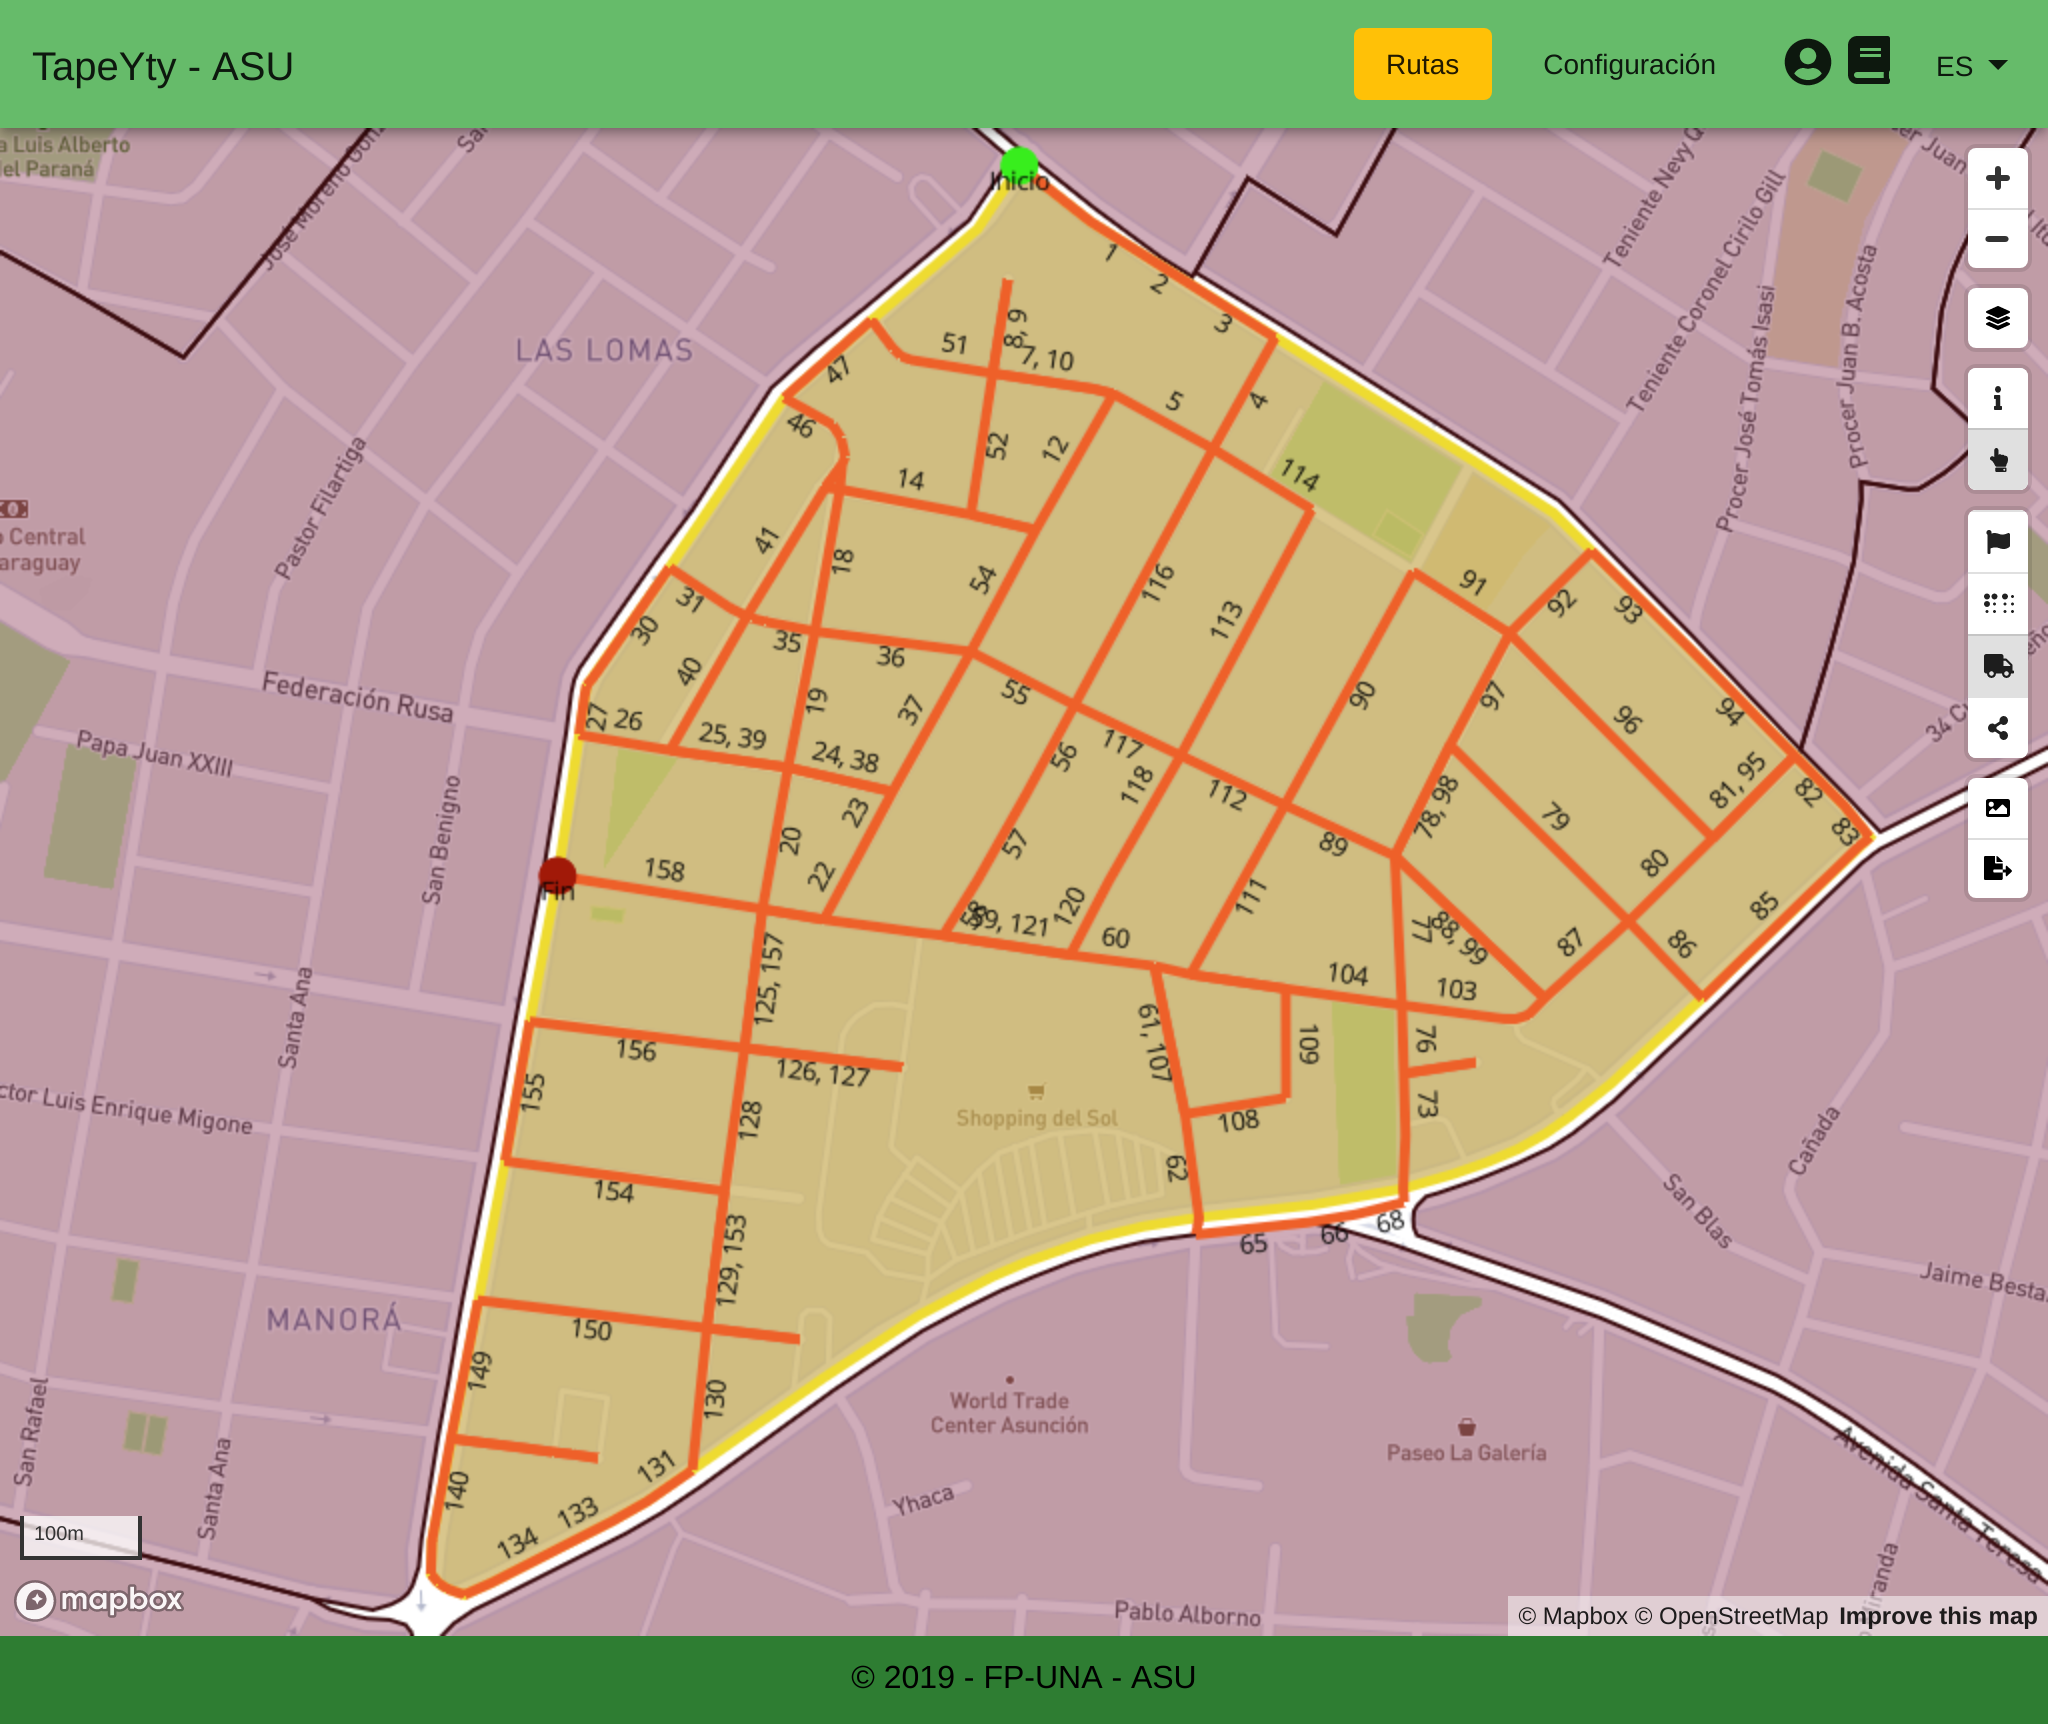
\includegraphics[width=0.85\textwidth]{imagenes/recorrido83ConOpcionales.png}}
\caption{Ruta generada por \textit{TapeYty} con la secuencia del camino indicada en cada arco.}
\label{fig:RecorridoTapeYtyZona83Opcionales}
\end{figure*}

Algunas zonas tienen varios segmentos de calles de un único sentido y si solo se utilizan los segmentos dentro de la zona, el resultado podría resultar infactible computacionalmente o más costoso en distancia, por ello se agrega una banda perimetral, tal como en \cite{Braier2017AnArgentina}, de 220 metros representada como segmentos opcionales (arcos auxiliares). Esta situación es común en la práctica actual de la recolección de residuos.

En la tabla \ref{table:comparacionZona83} se presenta el análisis realizado sobre la zona 83, los experimentos se ejecutan en una computadora personal con procesador Intel\textcopyright{}  Core\texttrademark{} i5 2.3 GHz, 7.7Gb de RAM, disco SSD y el sistema operativo Linux Mint en su version 18.3 Cinnamon 64-bit. En la primera columna se detallan las características de la zona, la segunda columna se refiere al escenario en el que todos los segmentos de calles deben ser visitados por el vehículo recolector y en la tercera columna se refiere al escenario en el que 6 segmentos de calles de sentido único y 3 de doble sentido fueron marcados como opcionales desde la aplicación. Ambos escenarios coinciden en la cantidad de vértices en el grafo, cantidad de calles de sentido único y de doble sentido, no así en la cantidad de arcos auxiliares, debido a la cantidad de segmentos opcionales. En el primer escenario es posible resolver mediante la técnica de mezcla de subtours recién en la segunda iteración, mientras que en el segundo se puede resolver con la misma técnica ya en la primera iteración, por ello se observa que el tiempo de ejecución del modelo es levemente menor para el segundo escenario. Realizar la expansión del grafo a partir de los datos de entrada es el paso que requirió de mayor tiempo en la aplicación. En ambos escenarios se redujo la distancia con respecto al recorrido actual, en el primero en un 20.31\% y en el segundo un 28.50\%, con 3.44105 km. y 4.82806 km. menos respectivamente.

% Please add the following required packages to your document preamble:
% \usepackage{multirow}
\begin{table}[htbp]
\caption{Resultados y análisis para la zona 83}
\begin{tabular}{lll}
\hline
\multirow{2}{*}{Zona 83}                            & \multicolumn{2}{l}{Cobertura de segmentos de calles} \\ \cline{2-3} 
                                                    & Sin opcionales           & Con opcionales           \\ \hline
$|V|$                                                   & 1352                     & 1352                     \\
$|E|$                                                   & 420                      & 420                      \\
$|AM|$                                                  & 256                      & 256                      \\
$|Aaux|$                                                & 1567                     & 1579                     \\
Iteraciones                                         & 2                        & 1                        \\
Tiempo de expansión (s)                      & 20.54530                 & 22.06926                 \\ 
Tiempo de ejecución de modelo (s)            & 0.52790                  & 0.31660                  \\ 
Tiempo de secuenciación (s)                  & 0.04023                  & 0.03425                  \\ 
Distancia (km)                                      & 13.49895                 & 12.11194                 \\ 
Mejor con respecto al actual (\%) & 20.31                    & 28.50                    \\ \hline
\end{tabular}
\label{table:comparacionZona83}
\end{table}

\section{Conclusión}

En ciudades en vías de desarrollo, como Asunción, el trayecto seguido por el conductor del vehículo de recolección de basura se basa en su propia intuición y experiencia debido a la falta de herramientas que ayuden a la toma de decisiones. Constantemente, las calles de Asunción sufren modificaciones como cambios de sentido e inhabilitación por diversos motivos; lo que requiere de un sistema flexible a estos cambios y pueda generar la ruta a seguir que contraste con la realidad del momento. Se propone un diseño de aplicación GIS cuyo principal objetivo es brindar el camino óptimo que debe seguirse para la recolección de residuos sólidos en las zonas.

Esta arquitectura propuesta tiene un factor muy relevante que es la escalabilidad al ofrecer componentes desacoplados, ya que se utilizan servicios REST, servicios web de mapas como \textit{TMS}, y \textit{fameworks} MVC. La metodología de trabajo en la DSU se ajusta al problema del ``Cartero Rural Abierto'', en este trabajo se utiliza la solución propuesta por \cite{Braier2017AnArgentina}, cuya salida representa los datos de entrada a la solución de secuenciación que finalmente se despliega en la aplicación.
%GIS.

La DSU podrá contar con una aplicación que garantice que todos los ciudadanos que residen e ingresan diariamente a la ciudad reciban el servicio de recolección de basura. Se evidencia que aunque se mantenga el procedimiento de recolección, la distancia del recorrido es mejorada y se observa que mediante el uso de la aplicación es posible reducir el número de veces que se pasa por los mismos segmentos de calles, además se garantiza que todos los segmentos serán cubiertos por la recolección.

El estudio podría ampliarse agregando el relieve del camino como un factor en la generación de ruta \cite{Sulemana2018OptimalMethods}, y compararla con el modelo implementado en este trabajo, teniendo en cuenta que el centro de la ciudad de Asunción y alrededores está levantada sobre 7 (siete) colinas.

Los autores proponen crear una mesa de trabajo con la DSU para estudiar la conveniencia de reorganizar las zonas de trabajo y sus horarios de recolección teniendo en cuenta factores como la cantidad de generación de residuos, densidad poblacional, capacidad del camión y la congestión del tránsito. También aprovechar la escalabilidad de la arquitectura implementada para agregar la gestión de residuos de grandes generadores, los llamados residuos de manejo especial, generados en los procesos productivos e instalaciones industriales y comerciales.

% analizar la factibilidad de seguir utilizando la solución en este trabajo, en caso de que no sea factible seguir utilizando un modelo exacto, incorporar una heurística al diseño de la propuesta.

% Para futuras sugerencias de trabajo, el parámetro de demanda se puede considerar incierto en el modelo y las otras metaheurísticas como la optimización de colonias de hormigas y el algoritmo genético se pueden probar para resolver el problema como un rival para SA.
% \section*{Agradecimientos}

% Los autores agradecen a la Dirección de Servicios Urbanos de la Municipalidad de Asunción por permitirnos participar del procedimiento de la gestión de recolección actual que se lleva a cabo en la dirección.

\bibliography{referencias}
\bibliographystyle{IEEEtran}

\vspace{12pt}
\end{document}
